
%%%%%%%%%%%%%%%%%%%%%%%%%%%%%%%%%%%%%%%%%
% Short Sectioned Assignment LaTeX Template Version 1.0 (5/5/12)
% This template has been downloaded from: http://www.LaTeXTemplates.com
% Original author:  Frits Wenneker (http://www.howtotex.com)
% License: CC BY-NC-SA 3.0 (http://creativecommons.org/licenses/by-nc-sa/3.0/)
%%%%%%%%%%%%%%%%%%%%%%%%%%%%%%%%%%%%%%%%%

%----------------------------------------------------------------------------------------
%	PACKAGES AND OTHER DOCUMENT CONFIGURATIONS
%----------------------------------------------------------------------------------------

\documentclass[paper=a4, fontsize=11pt]{scrartcl} % A4 paper and 11pt font size

% ---- Entrada y salida de texto -----

\usepackage[T1]{fontenc} % Use 8-bit encoding that has 256 glyphs
\usepackage[utf8]{inputenc}
%\usepackage{fourier} % Use the Adobe Utopia font for the document - comment this line to return to the LaTeX default

% ---- Idioma --------

\usepackage[spanish, es-tabla]{babel} % Selecciona el español para palabras introducidas automáticamente, p.ej. "septiembre" en la fecha y especifica que se use la palabra Tabla en vez de Cuadro

% ---- Otros paquetes ----

\usepackage{url} % ,href} %para incluir URLs e hipervínculos dentro del texto (aunque hay que instalar href)
\usepackage{amsmath,amsfonts,amsthm} % Math packages
%\usepackage{graphics,graphicx, floatrow} %para incluir imágenes y notas en las imágenes
\usepackage{graphics,graphicx, float} %para incluir imágenes y colocarlas
\usepackage{movie15}
\usepackage{pifont}
\usepackage{booktabs}
\usepackage{multirow}
\usepackage{rotating}
\usepackage[a4paper]{geometry}
\geometry{top=2.5cm, bottom=2.5cm, left=3cm, right=3cm}

% Para hacer tablas comlejas
%\usepackage{multirow}
%\usepackage{threeparttable}

%\usepackage{sectsty} % Allows customizing section commands
%\allsectionsfont{\centering \normalfont\scshape} % Make all sections centered, the default font and small caps

\usepackage{fancyhdr} % Custom headers and footers
\usepackage{tabularx}

\pagestyle{fancyplain} % Makes all pages in the document conform to the custom headers and footers
\fancyhead{} % No page header - if you want one, create it in the same way as the footers below
\fancyfoot[L]{} % Empty left footer
\fancyfoot[C]{} % Empty center footer
\fancyfoot[R]{\thepage} % Page numbering for right footer
\renewcommand{\headrulewidth}{0pt} % Remove header underlines
\renewcommand{\footrulewidth}{0pt} % Remove footer underlines
\setlength{\headheight}{13.6pt} % Customize the height of the header

\numberwithin{equation}{section} % Number equations within sections (i.e. 1.1, 1.2, 2.1, 2.2 instead of 1, 2, 3, 4)
\numberwithin{figure}{section} % Number figures within sections (i.e. 1.1, 1.2, 2.1, 2.2 instead of 1, 2, 3, 4)
\numberwithin{table}{section} % Number tables within sections (i.e. 1.1, 1.2, 2.1, 2.2 instead of 1, 2, 3, 4)

\setlength\parindent{0pt} % Removes all indentation from paragraphs - comment this line for an assignment with lots of text

\newcommand{\horrule}[1]{\rule{\linewidth}{#1}} % Create horizontal rule command with 1 argument of height
\usepackage[breaklinks=true]{hyperref}
\usepackage{cleveref}
\usepackage[table]{xcolor}
%\usepackage[dvipsnames]{xcolor}
\usepackage{amssymb}
\usepackage{color}
\usepackage{listings}
\usepackage{upgreek} % para poner letras griegas sin cursiva
\usepackage{cancel} % para tachar
\usepackage{mathdots} % para el comando \iddots
\usepackage{mathrsfs} % para formato de letra
\usepackage{stackrel} % para el comando \stackbin
\lstset{ %
language=C++,                % elegir el lenguaje del código
stringstyle=\color{blue}\ttfamily,,
basicstyle=\normalsize\ttfamily,       % el tamaño del font a usar para el código
numbers=left,                   % dónde poner los números de línea 
numberstyle=\footnotesize,      % tamaño de font usados para los números de línea 
stepnumber=1,                   % el paso de numeración
numbersep=5pt,                  % distancia del numero de línea y la línea
backgroundcolor=\color{white},  % color de fondo, para usarlo hay que agregar  \usepackage{color}
showspaces=false,               % mostrar espacios en blanco ?
showstringspaces=false,         % subrayar espacios con cadenas?   
 showtabs=false,                 % mostrar taba usando cadenas? 
frame=single,           			% enmarcar el código?  
tabsize=2,          				% sets default tabsize to 2 spaces?
keywordstyle=\color{MidnightBlue}\ttfamily\bfseries,
commentstyle=\color{OliveGreen}\ttfamily,
morecomment=[l][\color{OliveGreen}]{\#},
captionpos=b,           % sets the caption-position to bottom?
breaklines=true,        % sets automatic line breaking?
breakatwhitespace=false,    % sets if automatic breaks should only happen at whitespace ?
title=\lstname,
escapeinside={\%*}{*)}          % if you want to add a comment within your code
}

\lstset{literate=
  {á}{{\'a}}1 {é}{{\'e}}1 {í}{{\'i}}1 {ó}{{\'o}}1 {ú}{{\'u}}1
  {Á}{{\'A}}1 {É}{{\'E}}1 {Í}{{\'I}}1 {Ó}{{\'O}}1 {Ú}{{\'U}}1
  {à}{{\`a}}1 {è}{{\`e}}1 {ì}{{\`i}}1 {ò}{{\`o}}1 {ù}{{\`u}}1
  {À}{{\`A}}1 {È}{{\'E}}1 {Ì}{{\`I}}1 {Ò}{{\`O}}1 {Ù}{{\`U}}1
  {ä}{{\"a}}1 {ë}{{\"e}}1 {ï}{{\"i}}1 {ö}{{\"o}}1 {ü}{{\"u}}1
  {Ä}{{\"A}}1 {Ë}{{\"E}}1 {Ï}{{\"I}}1 {Ö}{{\"O}}1 {Ü}{{\"U}}1
  {â}{{\^a}}1 {ê}{{\^e}}1 {î}{{\^i}}1 {ô}{{\^o}}1 {û}{{\^u}}1
  {Â}{{\^A}}1 {Ê}{{\^E}}1 {Î}{{\^I}}1 {Ô}{{\^O}}1 {Û}{{\^U}}1
  {œ}{{\oe}}1 {Œ}{{\OE}}1 {æ}{{\ae}}1 {Æ}{{\AE}}1 {ß}{{\ss}}1
  {ű}{{\H{u}}}1 {Ű}{{\H{U}}}1 {ő}{{\H{o}}}1 {Ő}{{\H{O}}}1
  {ç}{{\c c}}1 {Ç}{{\c C}}1 {ø}{{\o}}1 {å}{{\r a}}1 {Å}{{\r A}}1
  {€}{{\EUR}}1 {£}{{\pounds}}1
  {ñ}{{\~n}}1
}

\hypersetup{
    colorlinks=true,
    linkcolor=black,
    filecolor=magenta,      
    urlcolor=blue,
    pdftitle={FFT: Prácticas - Mario Rodríguez Ruiz},
    bookmarks=true,
    citecolor=blue,
}



%----------------------------------------------------------------------------------------
%	TÍTULO Y DATOS DEL ALUMNO
%----------------------------------------------------------------------------------------

\title{	
\normalfont \normalsize 
\textsc{\textbf{Fundamentos físicos y tecnológicos (2016-2017)} \\ Subgrupo C1 \\ Grado en Ingeniería Informática\\ Universidad de Granada} \\ [25pt] % Your university, school and/or department name(s)
\horrule{0.5pt} \\[0.4cm] % Thin top horizontal rule
\huge Prácticas \\ % The assignment title
\horrule{2pt} \\[0.5cm] % Thick bottom horizontal rule
}

\author{Mario Rodríguez Ruiz} % Nombre y apellidos

\date{\normalsize\today} % Incluye la fecha actual

%----------------------------------------------------------------------------------------
% DOCUMENTO
%----------------------------------------------------------------------------------------

\begin{document}

\maketitle % Muestra el Título

\newpage %inserta un salto de página

\tableofcontents % para generar el índice de contenidos

\listoffigures

\listoftables

\newpage

%----------------------------------------------------------------------------------------
%	Cuestión 1
%----------------------------------------------------------------------------------------

\section{MANEJO DEL POLÍMETRO. MEDIDAS EN CONTINUA}

\subsection{Cuestiones teóricas}
	\subsubsection{Fuente de tensión}
		\begin{itemize}
			\item \textbf{\textit{Calcular la resistencia mínima que se puede colocar en los extremos de la fuente de tensión}}
			
			Resistencia mínima para que la corriente I que circula por el circuito sea menor que 1A (para $ V_{i}=5V $):			
			$ R = \dfrac{5V}{1A} \hspace{4pt} $ {\fboxrule=1pt \fboxsep=6pt
				\fbox{$ R = 5 \Omega $}}
			\\
			
			Resistencia mínima para que la corriente I que circula por el circuito sea menor que 0,5A (para $ V_{i}=15V $):			
			$ R = \dfrac{15V}{0,5A} \hspace{4pt} $ {\fboxrule=1pt \fboxsep=6pt
				\fbox{$ R = 30 \Omega $}}
			
			\item \textbf{\textit{¿Por qué no se debe utilizar una resistencia menor que la calculada?}}
			
			Si se utilizan resistencias menores a las calculadas para cada caso, se rebasarían las limitaciones de corriente de la fuente de tensión, lo que podría producir que se destruyeran componentes de ésta.
		\end{itemize}
	
	\subsubsection{Medida de tensiones}
		\begin{itemize}
			\item \textbf{\textit{¿Cómo debe ser esta resistencia R, para que el circuito no sea modificado por el voltímetro?}}
			
			La resistencia R del voltímetro debe debe tener un valor muy elevado
			para que pase la menor corriente posible por éste.
		\end{itemize}
	
	\subsubsection{Medida de intensidad}
		\begin{itemize}
			\item \textbf{\textit{¿Cómo debe ser la resistencia r, para que el circuito se modifique lo menos posible?}}
			
			La resistencia r del voltímetro debe debe tener un valor muy bajo
			para que no se note afectada la intensidad que circula por la rama.
			
			\item \textbf{\textit{¿Qué ocurre si se desea medir la corriente que circula por el circuito anterior, y por error, se hace
					como en la siguiente figura?}}
			
			Como se ha explicado antes, la resistencia en el amperímetro debe ser muy baja, por lo que casi toda la corriente pasaría por éste y se produciría un cortocircuito. La
			intensidad sería mayor de la que advierte el fabricante y, en consecuencia, se podría fundirse además el fusible.
			
			\item \textbf{\textit{¿Qué corriente circularía por el amperímetro?}}
			
			$ I_{r} = \dfrac{V_{i}}{r} = \dfrac{5V}{5\Omega} $ \hspace{5pt} {\fboxrule=1pt \fboxsep=6pt
				\fbox{$ I_{r} = 1A $}} Por lo que llegaría hasta 0,2A, que es lo que permite el fusible, y ya no pasaría más ya que éste se fundiría.
			
			\subsubsection{Medida de intensidad}
			Debe hacerse así porque si no la intensidad variará ya que se tendrán más elementos que estarán modificándola y habría que tenerlos en cuenta para los cálculos.
			
		\end{itemize}
\newpage

\subsection{Resistencias y medidas en continua}
\subsubsection{Valor nominal y valor medido}
\textbf{\textit{Coger 6 resistencias y crear una tabla con los valores medidos de las resistencias. Compararlos con
	con el valor nominal dado por el código de colores y comprobar que los valores medidos están dentro
	de la tolerancia especificada por el fabricante}}

\begin{table}[!hbt]
	\label{tablaejemplo}
	\begin{center}
		\begin{tabular}{|c|c|c|c|c|}
			\hline
			\textbf{Nombre} & \textbf{Colores} & \textbf{V. Nominal y tolerancia} & \textbf{V. Medido} & \textbf{¿Cumple?} \\
			\hline
			R1 & VE-AZ-AM-O 	& $ 56 \times 10^{4} \Omega \pm 5\% $ & $ 566 k\Omega $ & SI \\
			R2 & MA-MA-NE-RO-VI & $ 110 \times 10^{2} \Omega \pm 0,1\% $ & $ 10,99 k\Omega $ 	& SI \\
			R3 & MA-VE-RO-O 	& $ 15 \times 10^{2} \Omega \pm 5\% $ & $ 1,495 k\Omega $ & SI \\
			R4 & VE-AZ-RO-O 	& $ 56 \times 10^{2} \Omega \pm 5\% $ & $ 5,47 k\Omega $ & SI \\
			R5 & MA-RO-MA-O 	& $ 12 \times 10^{1} \Omega \pm 5\% $ & $ 118,5 \Omega $ & SI \\
			R6 & RO-NE-NA-O 	& $ 20 \times 10^{3} \Omega \pm 5\% $ & $ 19,73 k\Omega $ & SI \\
			\hline
		\end{tabular}
		\caption[Tabla de Ejemplo]{Características de las resistencias.}
	\end{center}
\end{table}

\subsubsection{Agrupación de resistencias. Medidas en un circuito}

\begin{enumerate}
	\item \textbf{\textit{Montaje del circuito.}}
	
		\textbf{\textit{Se ha de montar la agrupación de 6 resistencias como el de la Figura \ref{fig:figura1}.}}
		
		\begin{figure}[H] %con el [H] le obligamos a situar aquí la figura
			\centering
			\includegraphics[scale=0.4]{capturas/figura1.png} 
			\caption{Circuito a montar}
			\label{fig:figura1}
		\end{figure}
		\begin{figure}[H] %con el [H] le obligamos a situar aquí la figura
			\centering
			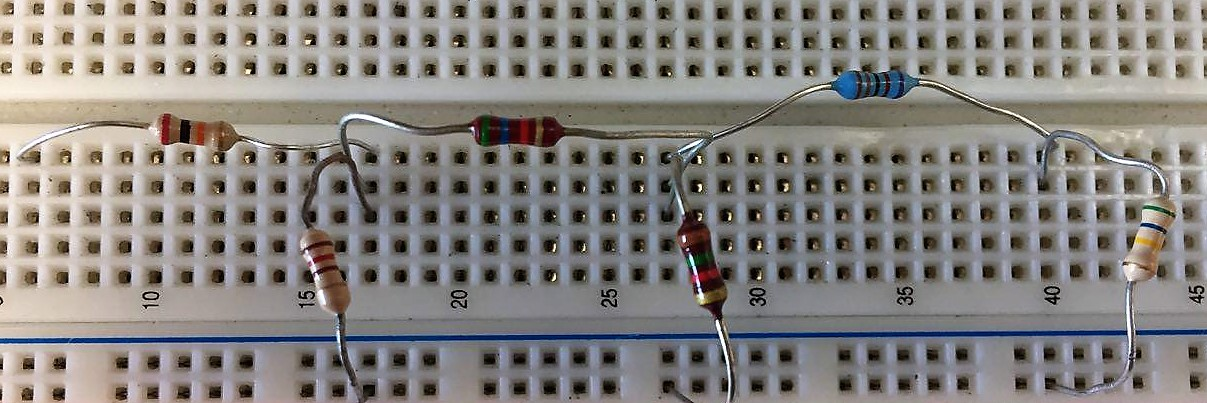
\includegraphics[scale=0.45]{capturas/figura2.jpg} 
			\caption{Circuito montado en la práctica 1}
			\label{fig:figura2}
		\end{figure}
	
	\item \textbf{\textit{Medir con el óhmetro la resistencia equivalente de la agrupación de resistencias.}}	
		\begin{center}
			{\fboxrule=1pt \fboxsep=6pt
				\fbox{$R_{e q} = 19,86 k\Omega$}}
		\end{center}
	
	\item \textbf{\textit{Calcular teóricamente (con los valores medidos de las resistencias) el valor de la agrupación.}}
		\begin{center}
			$ R_{A} =  R_{1} + R_{2} = 566 k\Omega + 10,99 k\Omega = 576,99 k\Omega$
			\\
			
			$ R_{B} =  \dfrac{R_{3} \cdot R_{A}}{R_{3} + R_{A}} = \dfrac{1,495 k\Omega \cdot 576,99 k\Omega}{1,495 k\Omega + 576,99 k\Omega} = 1,49 k\Omega$
			\\
			
			$ R_{C} =  R_{4} + R_{B} = 5,47 k\Omega + 1,49 k\Omega = 6,96 k\Omega$
			\\
			
			$ R_{D} =  \dfrac{R_{5} \cdot R_{C}}{R_{5} + R_{C}} = \dfrac{118,5 \Omega \cdot 6,96 k\Omega}{118,5 \Omega + 6,96 k\Omega} = 117 \Omega$
			\\
			
			$ R_{e q} =  R_{6} + R_{D} = 19,73 k\Omega + 117 \Omega $ 
			
			\begin{center}			
				{\fboxrule=1pt \fboxsep=6pt
					\fbox{$R_{e q} = 19,85 k\Omega$}}
			\end{center}
		\end{center}	
	
	\item \textbf{\textit{Medida indirecta de la Resistencia Equivalente.}}
	
		$V_{i} = 30,17 \hspace{5pt}V  $
		
		$I_{i} = 1,512 \hspace{5pt}mA $
		
		$R_{e q} = \dfrac{V_{i}MEDIDA}{I_{i}MEDIDA} =  \dfrac{30,17 \hspace{5pt}V}{1,512 \cdot 10^{-3} \hspace{5pt}A} $ \hspace{10pt}
		\fboxrule=1pt \fboxsep=6pt
		\fbox{$ R_{e q} = 19,95 k\Omega$}
	
	\item \textbf{\textit{Medir $ V_{R1} $, $ V_{R2} $, $ V_{R3} $ y $ V_{R5} $}}
	
	\begin{center}
		$ V_{R1} = 37,1 \hspace{5pt}mV$ \hspace{10pt} $ V_{R3} = 37,8 \hspace{5pt}mV$
	
		$ V_{R2} = 0,7 \hspace{5pt}mV$ \hspace{10pt} $ V_{R5} = 177,1 \hspace{5pt}mV$
	\end{center}
	
	\item \textbf{\textit{Calcular teóricamente $ V_{R1} $, $ V_{R3} $ y $ V_{R5} $}}
	
	A partir de la Fórmula del Partidor de Tensión:
	
	$ V_{R1} = V_{R3} \cdot \dfrac{R_{1}}{R_{1} + R_{2}} = 37,8 \hspace{5pt}mV \cdot \dfrac{566 k\Omega}{566 k\Omega + 10,99 k\Omega}$ \hspace{15pt} \fboxrule=1pt \fboxsep=6pt
	\fbox{$ V_{R1} = 37,08 \hspace{5pt}mV$}
	
	$ V_{R3} = V_{R5} \cdot \dfrac{R_{B}}{R_{4} + R_{B}} = 177,1 \hspace{5pt}mV \cdot \dfrac{1,49 k\Omega}{5,47 k\Omega + 1,49 k\Omega}$ \hspace{10pt} \fboxrule=1pt \fboxsep=6pt
	\fbox{$ V_{R3} = 37,91 \hspace{5pt}mV$}
	
	$ V_{R5} = V_{i} \cdot \dfrac{R_{D}}{R_{D} + R_{6}} = 30,17 \hspace{5pt}V \cdot \dfrac{0,117 k\Omega}{0,117 k\Omega + 19,73 k\Omega}$ \hspace{16pt} \fboxrule=1pt \fboxsep=6pt
	\fbox{$ V_{R5} = 177,86 \hspace{5pt}mV$}
	\vspace{10pt}
	\item \textbf{\textit{Medir (si es posible) $ I_{1} $ y calcularla teóricamente. }}
	
	$ I_{1}MEDIDA = 0,064 \hspace{5pt} \mu A $
	
	Cálculo teórico:
	
	$ I_{1} = \dfrac{V_{R1}}{R_{1}} = \dfrac{37,08 \cdot 10^{-3}\hspace{5pt}V}{566 \cdot 10^{3}\Omega} $ \hspace{2pt} \fboxrule=1pt \fboxsep=6pt
	\fbox{$ I_{1} = 0,0655 \hspace{5pt} \mu A = I_{2} $} \hspace{2pt} $ \dfrac{0,7 \cdot 10^{-3}\hspace{5pt}V}{10,99 \cdot 10^{3}\Omega} = \dfrac{V_{R2}}{R_{2}} = I_{2}  $
	
\end{enumerate}

\subsubsection{Cálculo del coeficiente de variación de resistencia con la temperatura ($ \alpha $)}

\begin{center}
	\fboxrule=1pt \fboxsep=6pt
\fbox{$ R_{(T)} = R_{(T_{0})}\cdot[1+\alpha(T-T_{0})] $}
\end{center}

$ R_{(T_{0})} = R_{FRIA} = 3,6 \Omega$ \hspace{10pt} $ T_{0} = 22^{o} = 295,15k $

$ I_{APUNTADA} = 0,28 A$

$ V_{MEDIDA} = 12,14 V$

$ R_{(T)} = R_{CALIENTE} = \dfrac{V_{MEDIDA}}{I_{APUNTADA}} = \dfrac{12,14 V}{0,28 A} $ \hspace{6pt} \fboxrule=1pt \fboxsep=6pt\fbox{$ R_{(T)} = 43,36 \Omega $}

$ P_{CONSUMIDA} = I_{APUNTADA} \cdot V_{MEDIDA} = 12,14 V \cdot 0,28 A $ \hspace{2pt} \fboxrule=1pt \fboxsep=6pt\fbox{$ P_{CONSUMIDA} = 3,399 W $}

Ley de Stefan: \fboxrule=1pt \fboxsep=6pt
\fbox{$ P = e \cdot \sigma \cdot A \cdot T^{4} $} $ \cong P_{RADIADA} $
\vspace{6pt}

$ T^{4} = \dfrac{P_{CONSUMIDA}}{e \cdot \sigma \cdot A} = \dfrac{3,399W}{1 \cdot 5,6704 \cdot 10^{-8} \frac{W}{m^{2}\cdot k^{4}} \cdot 2,6 \cdot 10^{-6}m^{2}} = \dfrac{3,399k^{4}}{1,47\cdot 10^{-13}}$ \hspace{2pt} \fboxrule=1pt \fboxsep=6pt\fbox{$ T = 2191,41k $}
\vspace{10pt}

Por tanto:
\vspace{10pt}

$ 43,36 \Omega = 3,6 \Omega \cdot [ 1 + \alpha (2191,41k - 295,15k)] $ \hspace{6pt} ; $ 1 + 1896,26k \cdot \alpha = \dfrac{43,36 \Omega}{3,6\Omega} $
\vspace{10pt}

$ 1896,26k \cdot \alpha = 12,04 - 1 $ \hspace{4pt} \fboxrule=1pt \fboxsep=6pt\fbox{$ \alpha = 5,82\cdot10^{-3}k^{-1} $}\\

Según la web de GoodFellow (empresa de venta de metales para investigación \url{http://www.goodfellow.com/S/Tungsteno.html}) el coeficiente de variación de resistencia con la temperatura del wolframio es de \textbf{$ 4,8 \cdot10^{-3}k^{-1} $}. Sin embargo, en wikipedia (\url{https://es.wikipedia.org/wiki/Coeficiente_de_temperatura}) expresan su valor como 

\textbf{$ 4,5\cdot10^{-3}k^{-1} $}.

La diferencia está en que en clase se ha calculado en base a $ 22^{o}C $ mientras que en \textbf{wikipedia}, por ejemplo, lo han hecho sobre $ 20^{o}C $.

\subsubsection{Calcular la longitud de onda $ \lambda_{MAX} $ a la cual, la bombilla emite la máxima radiación.}

Ley de desplazamiento de Wien: \fboxrule=1pt \fboxsep=6pt\fbox{$ \lambda_{MAX} \cdot T = 2897768,5 nm\cdot k$}\\
\vspace{6pt}

$ \lambda_{MAX} = \dfrac{2897768,5 nm\cdot k}{2191,41 k} $ \hspace{4pt} \fboxrule=1pt \fboxsep=6pt\fbox{$ \lambda_{MAX} = 1322,33 nm $}

\subsubsection{¿A qué "color" corresponde lMAX?}

Al estar $ \lambda_{MAX} $ por encima de los 700nm su color será el \textbf{infrarrojo}.

\newpage


\section{ALTERNA. AMPLIFICADOR OPERACIONAL. BODE}

\subsection{Medidas en Alterna}
\textbf{\textit{Medir con el osciloscopio la amplitud, periodo y frecuencia de dos señales generadas por el oscilador.
		Una debe ser triangular, y la otra cuadrada, sus amplitudes y frecuencias deben ser distintas.}}
% Table generated by Excel2LaTeX from sheet ,Hoja1,
\begin{table}[H]
	\centering
	\begin{tabular}{rcl|l|l|}
		&       & \multicolumn{1}{l}{\textcolor[rgb]{ .267,  .329,  .416}{\textbf{Señal:}}} & \multicolumn{1}{l}{\textcolor[rgb]{ .267,  .329,  .416}{\textbf{Triangular}}} & \multicolumn{1}{l}{\textcolor[rgb]{ .267,  .329,  .416}{\textbf{Cuadrada}}} \\
		\cmidrule{3-5}    \multirow{3}[2]{*}{\textcolor[rgb]{ .267,  .329,  .416}{\begin{sideways}\textbf{FTE}\end{sideways}}} & \multicolumn{1}{l}{\multirow{3}[2]{*}{\textcolor[rgb]{ .267,  .329,  .416}{\begin{sideways}\textbf{SEÑAL}\end{sideways}}}} & Amplitud & 3,5 V & 5,5 V \\
		&       & Periodo & 200 $ \mu $s & 400 $ \mu $s \\
		&       & Frecuencia & 5 kHz & 2,5 kHz \\
		\cmidrule{1-2}    \multirow{9}[6]{*}{\textcolor[rgb]{ .267,  .329,  .416}{\begin{sideways}\textbf{OSCILOSCOPIO}\end{sideways}}} & \multirow{3}[2]{*}{\textcolor[rgb]{ .267,  .329,  .416}{\begin{sideways}\textbf{DIV}\end{sideways}}} & Amplitud & 6,875 div · 0,5 V/div = 3,438 V & 5,45 div · 1 V/div =  5,45 V \\
		&       & Periodo & 4 div · 50 $ \mu $s/div = 200 $ \mu $s & 2 div · 198 $ \mu $s/div = 396 $ \mu $s \\
		&       & Frecuencia & 5 kHz & 2,53 kHz \\
		\cmidrule{2-2}          & \multirow{3}[2]{*}{\textcolor[rgb]{ .267,  .329,  .416}{\begin{sideways}\textbf{CUR}\end{sideways}}} & Amplitud & 3,438 V & 5,438 V \\
		&       & Periodo & 200 $ \mu $s & 400 $ \mu $s \\
		&       & Frecuencia & 5 kHz & 2,5 kHz \\
		\cmidrule{2-2}          & \multirow{3}[2]{*}{\textcolor[rgb]{ .267,  .329,  .416}{\begin{sideways}\textbf{AUTO}\end{sideways}}} & Amplitud & 3,438 V & 5,438 V \\
		&       & Periodo & 200 $ \mu $S & 400 $ \mu $s \\
		&       & Frecuencia & 5 kHz & 2,5 kHz \\
		\cmidrule{1-2}    \end{tabular}%
	\caption{Medidas en Alterna}
	\label{tab:addlabel}%
\end{table}%


\subsection{Filtro con amplificador operacional. Diagrama de Bode}

\renewcommand{\labelitemi}{\ding{42}}
\begin{itemize}
	\item \textbf{\textit{Construir el filtro pasobaja (LP) que se muestra en la Figura \ref{fig:figura3}. La frecuencia de corte del filtro (fc)
	deberá ser 2 kHz.
	La ganancia de la etapa coincide con k=(1+$ R_{2} $/$ R_{1} $ )=2 (usar dos resistencias iguales).}}
	
		\begin{figure}[H] %con el [H] le obligamos a situar aquí la figura
			\centering
			\includegraphics[scale=0.4]{capturas/figura3.png} 
			\caption{Filtro con amplificador operacional teórico}
			\label{fig:figura3}
		\end{figure}
	\vspace{-19pt}
		La Figura \ref{fig:figura5} muestra la resistencia elegida para componer los lugares que ocuparán $ R_{1} $ y $ R_{2} $.
		
		\begin{figure}[H] %con el [H] le obligamos a situar aquí la figura
			\centering
			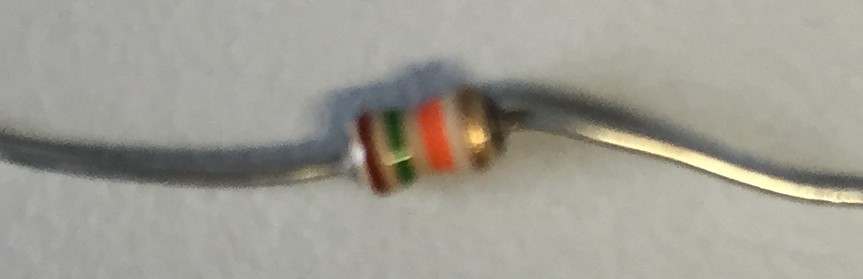
\includegraphics[scale=0.3]{capturas/R1YR2.jpg} 
			\caption{Filtro con amplificador operacional construido}
			\label{fig:figura5}
		\end{figure}
		
		$ R_{1MEDIDA} = 14,89 k\Omega $
		
		$ R_{2MEDIDA} = 14,92 k\Omega $ 
		
		$ k_{real} = (1 + \dfrac{R_{2MEDIDA}}{R_{1MEDIDA}}) = (1 + \dfrac{14,92 k\Omega}{14,89 k\Omega})$
		
		\begin{center}			
			{\fboxrule=1pt \fboxsep=6pt
				\fbox{$ k_{real} = 2,002 $}}
		\end{center}
	
		La Figura \nameref{fig:figura4} muestra la construcción en laboratorio del filtro pasobaja (LP)
	
		\begin{figure}[H] %con el [H] le obligamos a situar aquí la figura
			\centering
			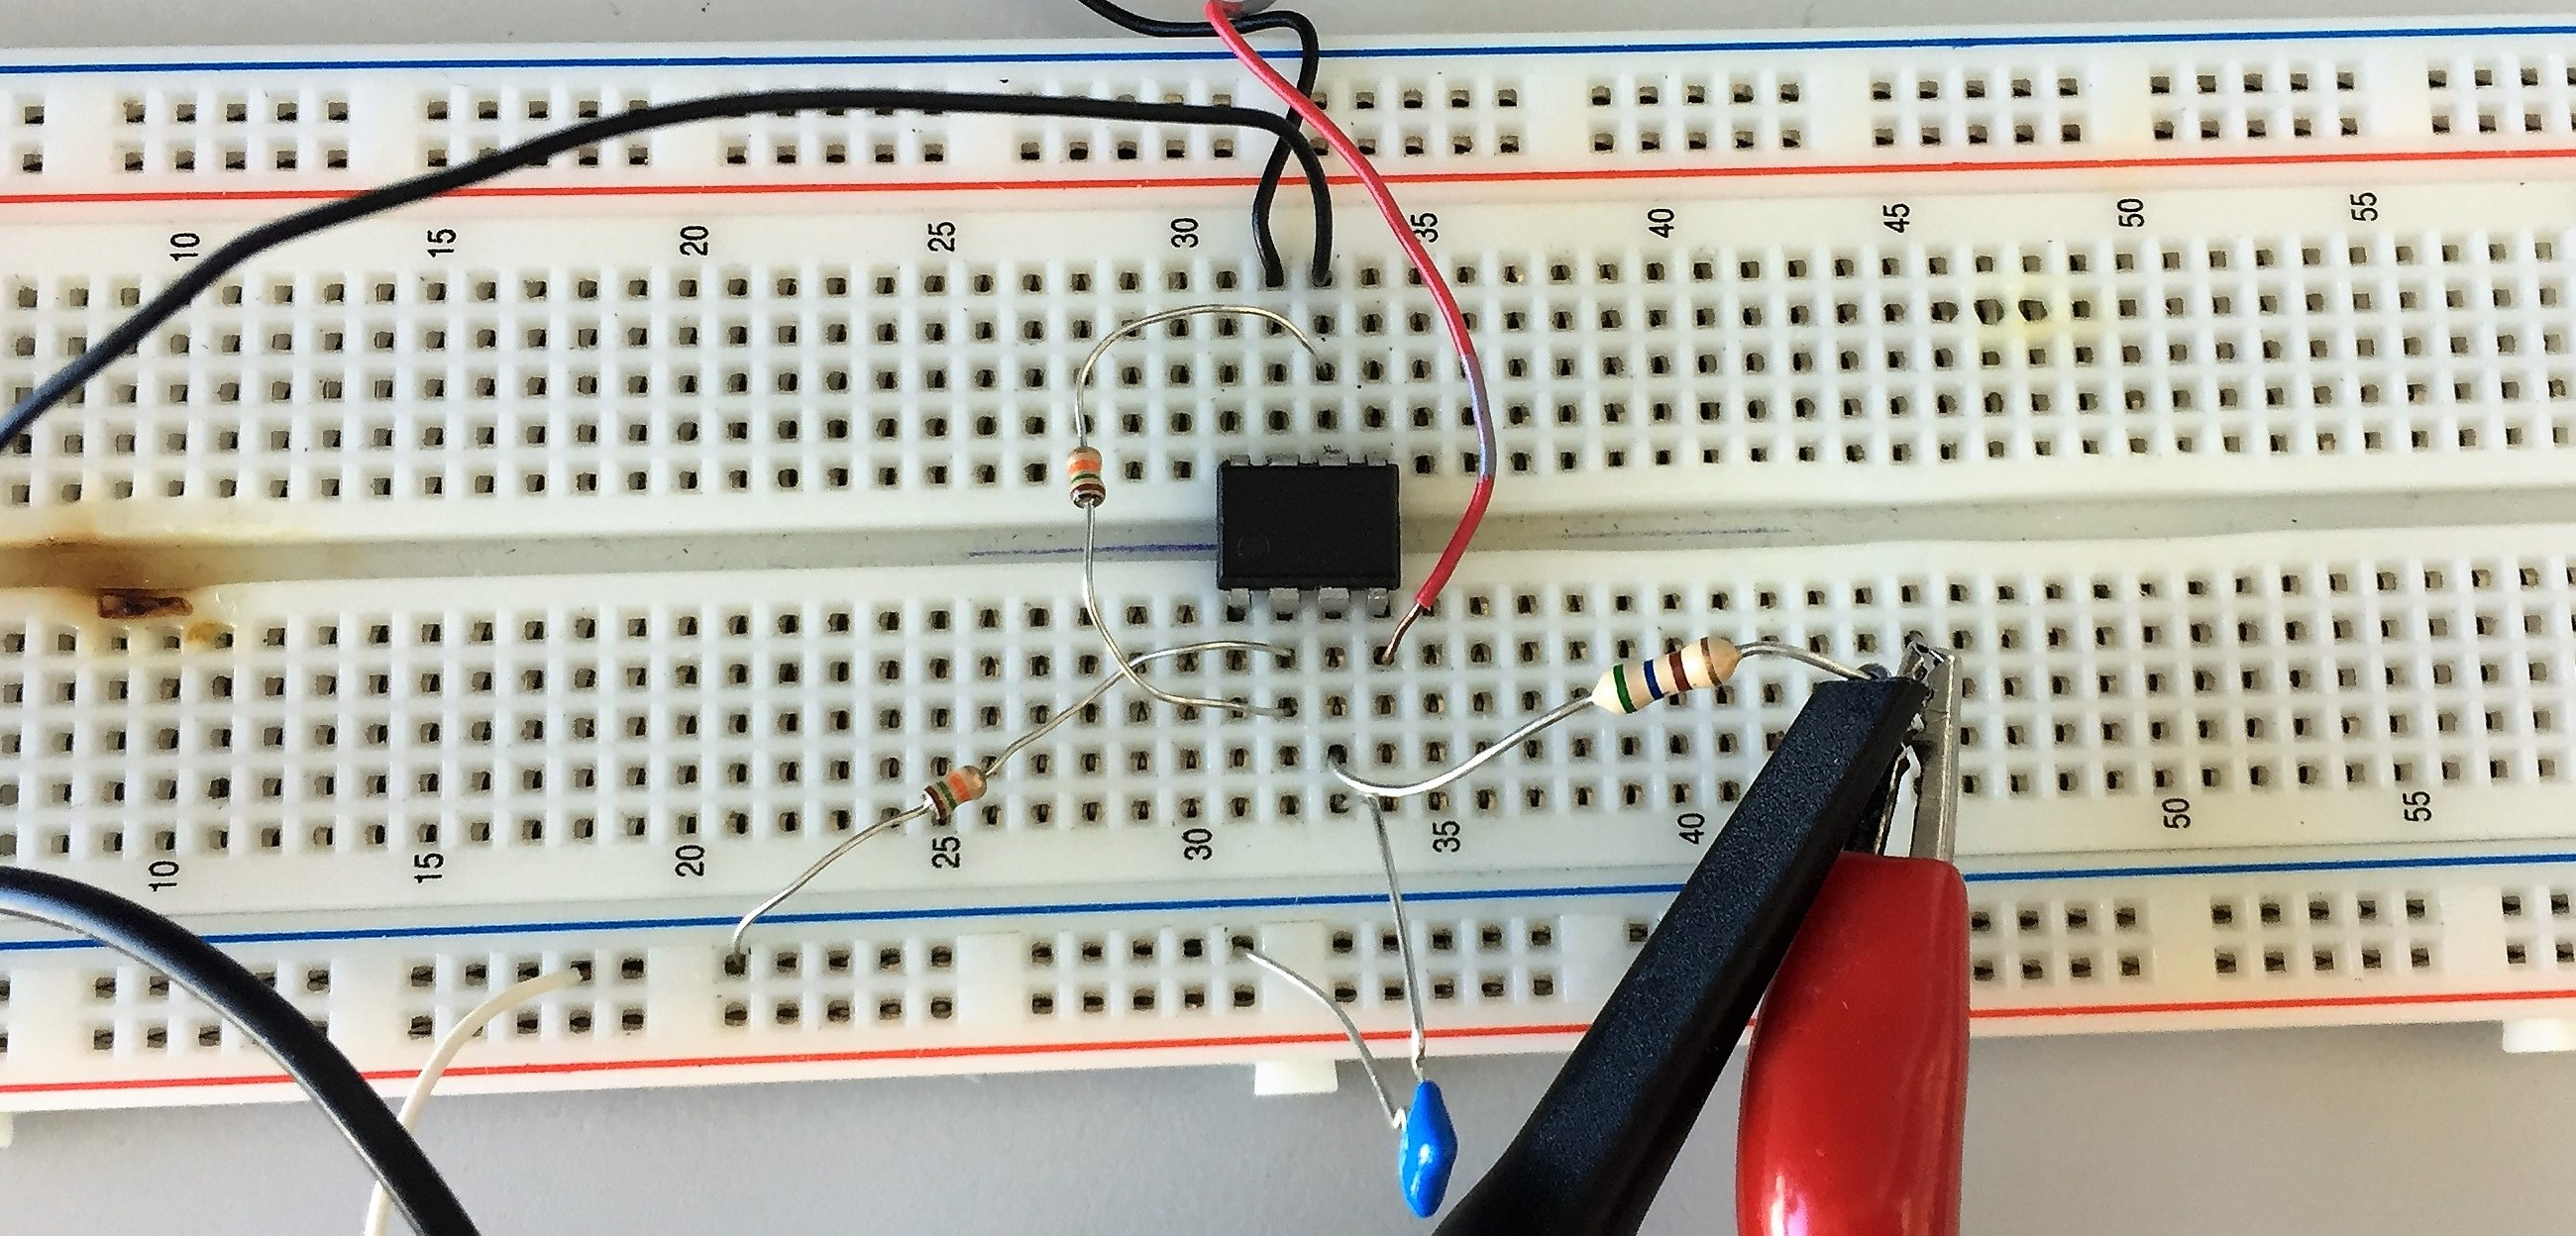
\includegraphics[scale=0.15]{capturas/figura4.jpg} 
			\caption{Filtro con amplificador operacional construido}
			\label{fig:figura4}
		\end{figure}		

	\item \textbf{\textit{Indique los valores cogidos de R, C y $ f_{C} $, y el proceso seguido para su elección}}.
	
		El condensador escogido en laboratorio es el de la Figura \ref{fig:figura6} y su valor es:
		\begin{center}			
			{\fboxrule=1pt \fboxsep=6pt
				\fbox{$ C = 147 nF $}}
		\end{center}		
		
		\begin{figure}[H] %con el [H] le obligamos a situar aquí la figura
			\centering
			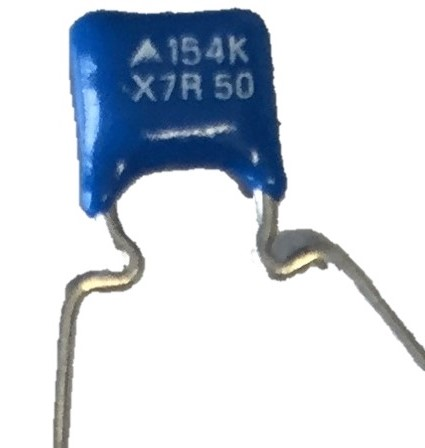
\includegraphics[scale=0.3]{capturas/C.jpg} 
			\caption{Condensador para el Filtro con amplificador operacional}
			\label{fig:figura6}
		\end{figure}
	
		$ w_{C} = 2\pi\cdot f_{C} = \dfrac{1}{R \cdot C} $
		
		Frecuencia de corte $= f_{C} = 2 kHz $
		
		\begin{align*}
			R& ? 	&	w_{C} &= 2\pi \cdot 2000Hz = \dfrac{1}{R \cdot 147 \cdot 10^{-9}F}\\		
			R &= \dfrac{1}{2\pi \cdot 2000Hz \cdot 147 \cdot 10^{-9}F} 		& R & = 541,34 \Omega 
		\end{align*}

		Con el resultado obtenido de R, la resistencia más apropiada para elegir en el laboratorio según estas necesidades es la de la Figura \ref{fig:figura7} que es de $ 561\Omega $ aproximadamente.
		
		\begin{figure}[H] %con el [H] le obligamos a situar aquí la figura
			\centering
			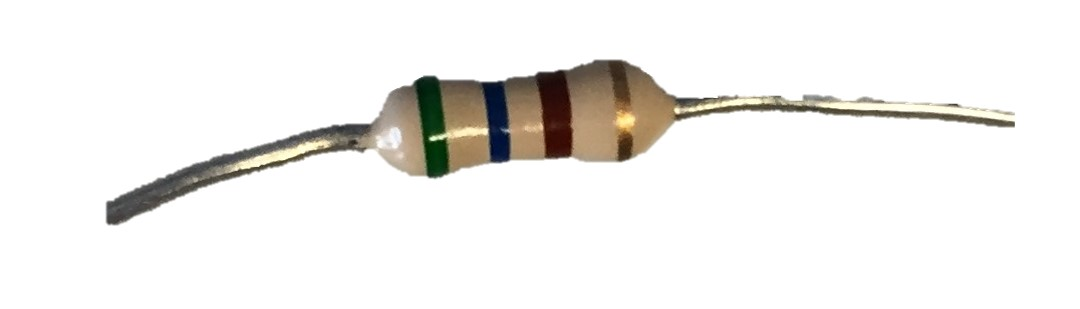
\includegraphics[scale=0.4]{capturas/R.jpg} 
			\caption{Resistencia R del Filtro operacional}
			\label{fig:figura7}
		\end{figure}
	
		Con todos los componentes ya seleccionados es el momento del montaje completo del circuito y de conectar los distintos canales del osciloscopio, del oscilador y de la fuente de tensión sobre él, tal y como indica la guía de la Figura \ref{fig:figura8}
		
		\begin{figure}[H] %con el [H] le obligamos a situar aquí la figura
			\centering
			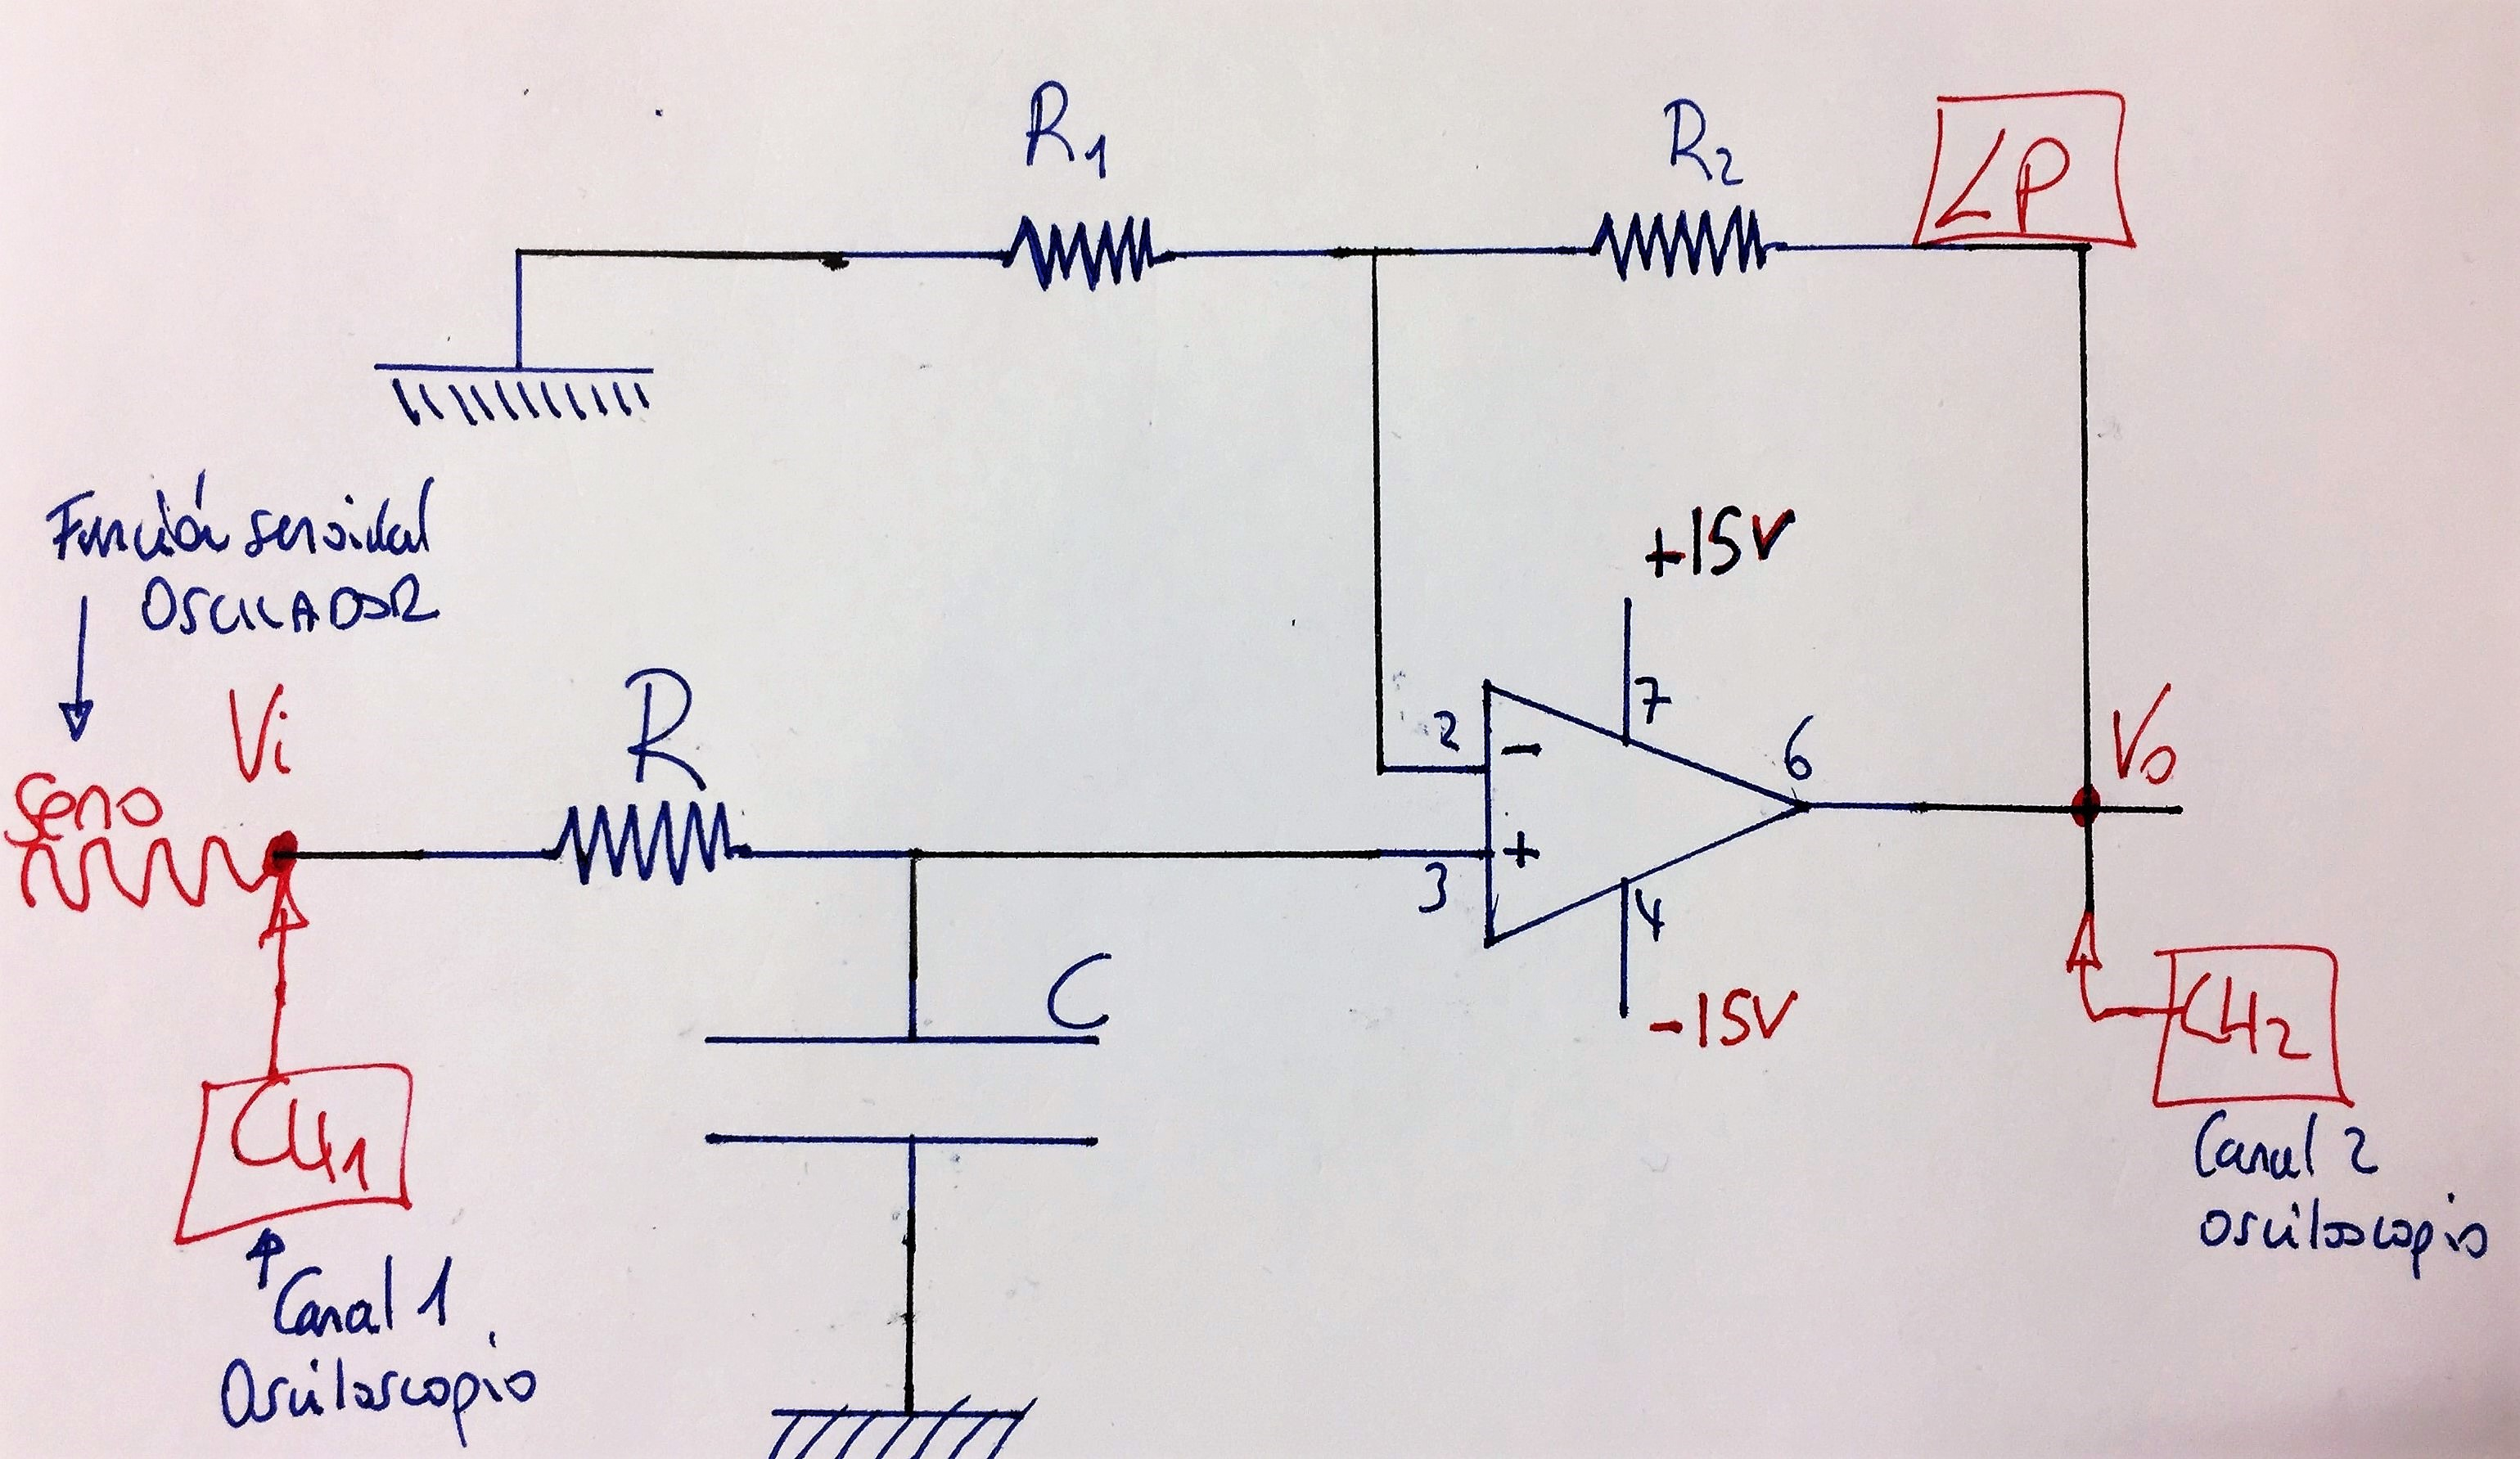
\includegraphics[scale=0.13]{capturas/circ.jpg} 
			\caption{Filtro operacional}
			\label{fig:figura8}
		\end{figure}
	
		El resultado del montaje final antes de proceder a tomar las medidas es el de la Figura \ref{fig:figura9}
		
		\begin{figure}[H] %con el [H] le obligamos a situar aquí la figura
			\centering
			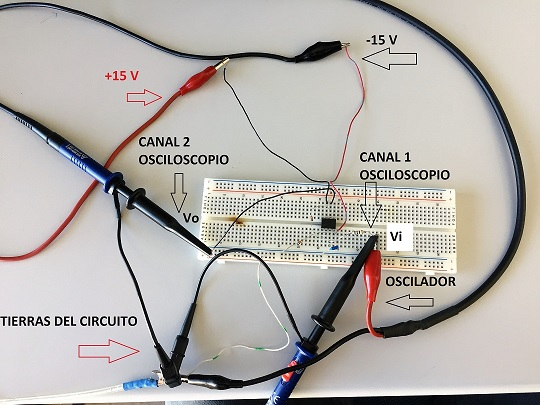
\includegraphics[scale=0.7]{capturas/final.jpg} 
			\caption{Filtro operacional}
			\label{fig:figura9}
		\end{figure}
	
	\item \textbf{\textit{Inmediatamente tras construir la etapa, debe comprobarse lo siguiente:}}
		\begin{itemize}
			\item [$ - $]\textbf{\textit{La ganancia a bajas frecuencias en el pasobaja, debe ser igual a k=(1+R2/R1). Debería salir
			aproximadamente igual a 2 (6 dB).}}			
				\begin{align*}
					 f &= 200 Hz & ; &	& V_{o} &= 12,5V & ; & & V_{i} &= 6,25V & ; & &	\dfrac{V_{o}}{V_{i}} &= \dfrac{12,5V}{6,25V} = 2					 	
				\end{align*}
				
			\item [$ - $]\textbf{\textit{La frecuencia de corte $ f_{c} $=1/(2p·RC) está próxima a la teórica (según los valores de R y C escogidos).
					La frecuencia de corte es aquélla en la que la ganancia es k/$ \sqrt{2} $=0,707·k (caída de 3 dB). En nuestro
					caso, debería salir aproximadamente 2/$ \sqrt{2} $=$ \sqrt{2} $=1,4142 (3 dB, que es 6 dB menos la caída de 3 dB)}}			
				\begin{align*}
				f &= 2 kHz & ; &	& V_{o} &= 7,81V & ; & & V_{i} &= 5,88V & ; & &	\dfrac{V_{o}}{V_{i}} &= \dfrac{7,81V}{5,88V} = 1,33					 	
				\end{align*}
				
			\item [$ - $]\textbf{\textit{La ganancia a 10·$ f_{c} $ en el filtro pasobaja debería salir aproximadamente igual a k/10=2/10=0,2 (-14 dB,
					que es 20 dB menos que la máxima ganancia de 6 dB)}}			
				\begin{align*}
					f &= 20 kHz & ; &	& V_{o} &= 1,13V & ; & & V_{i} &= 5,69V & ; & &	\dfrac{V_{o}}{V_{i}} &= \dfrac{1,13V}{5,69V} = 0,199					 	
				\end{align*}
		\end{itemize}
	\newpage
		\item \textbf{\textit{Diagrama de Bode}}
		
		% Table generated by Excel2LaTeX from sheet ,Hoja1,
		\begin{table}[htbp]
			\centering
			\begin{tabular}{rrrrr}
				\rowcolor[rgb]{ .839,  .863,  .894} \multicolumn{1}{l}{\textbf{f (Hz)}} & \multicolumn{1}{l}{\textbf{Vi (V)}} & \multicolumn{1}{l}{\textbf{Vo (V)}} & \multicolumn{1}{l}{\textbf{Vo/Vi}} & \multicolumn{1}{l}{\textbf{20log(Vo/Vi) (dB)}} \\
				20    & 6,25  & 12,5  & 2     & 6,020599913 \\
				30    & 6,25  & 12,5  & 2     & 6,020599913 \\
				80    & 6,25  & 12,5  & 2     & 6,020599913 \\
				150   & 6,25  & 12,5  & 2     & 6,020599913 \\
				200   & 6,25  & 12,5  & 2     & 6,020599913 \\
				210   & 6,35  & 12,5  & 1,968503937 & 5,882725754 \\
				230   & 6,25  & 12,5  & 2     & 6,020599913 \\
				250   & 6,25  & 12,3  & 1,968 & 5,880501882 \\
				300   & 6,25  & 12,2  & 1,952 & 5,809596267 \\
				500   & 6,25  & 11,9  & 1,904 & 5,593338881 \\
				700   & 6,19  & 11,4  & 1,841680129 & 5,304284046 \\
				900   & 6,19  & 10,9  & 1,760904685 & 4,914716978 \\
				1100  & 6     & 10,2  & 1,7   & 4,608978428 \\
				1500  & 6     & 9,1   & 1,516666667 & 3,617802839 \\
				2000  & 5,88  & 7,81  & 1,328231293 & 2,465474156 \\
				2500  & 5,88  & 6,81  & 1,158163265 & 1,275395717 \\
				3000  & 5,88  & 6,06  & 1,030612245 & 0,261905962 \\
				4000  & 5,75  & 4,88  & 0,848695652 & -1,424960454 \\
				6000  & 5,69  & 3,41  & 0,599297012 & -4,447157748 \\
				8000  & 5,69  & 2,63  & 0,462214411 & -6,703130358 \\
				10000 & 5,69  & 2,11  & 0,370826011 & -8,616596222 \\
				11000 & 5,69  & 1,95  & 0,342706503 & -9,301553101 \\
				13000 & 5,69  & 1,67  & 0,293497364 & -10,6479159 \\
				16000 & 5,69  & 1,36  & 0,239015817 & -12,43146716 \\
				18000 & 5,69  & 1,25  & 0,219683656 & -13,16404507 \\
				20000 & 5,69  & 1,13  & 0,198594025 & -14,04067646 \\
				22000 & 5,69  & 1,02  & 0,179261863 & -14,93024189 \\
				26000 & 5,69  & 0,875 & 0,153778559 & -16,26208427 \\
				33000 & 5,69  & 0,725 & 0,12741652 & -17,8954852 \\
				38000 & 5,69  & 0,637 & 0,111950791 & -19,01945668 \\
			\end{tabular}%		
			\caption{Frecuencias desde 80Hz hasta 50kHz}
			\label{tab:frecuencias}%
		\end{table}%		
	
	\begin{figure}[H] %con el [H] le obligamos a situar aquí la figura
		\centering
		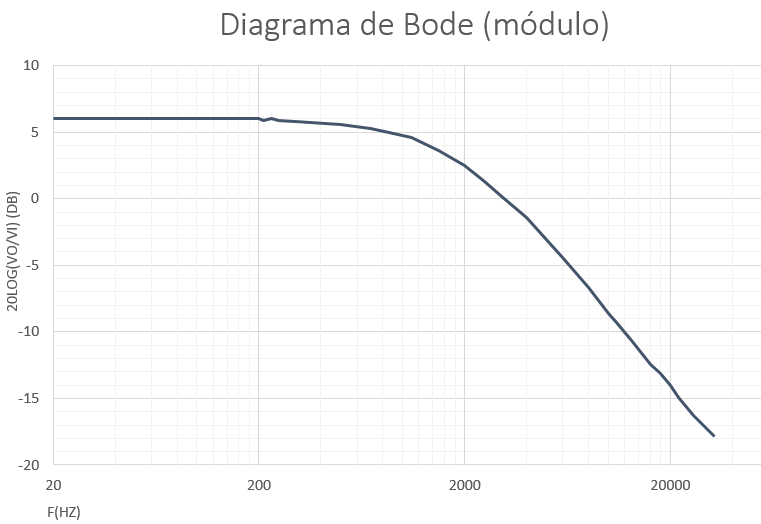
\includegraphics[scale=0.8]{capturas/bode.png} 
		\caption{Diagrama de Bode}
		\label{fig:bode}
	\end{figure}
\end{itemize}

\section{DIODO. UNIÓN PN}

\subsection{Polarización directa. Tensión umbral (V$ \gamma $) y resistencia dinámica ($ r_{d} $)}

$ r_{d} = (V_{d-max}-V\gamma)/I_{d-max} $
% Table generated by Excel2LaTeX from sheet ,Hoja1,
\begin{table}[H]
	\centering
	\begin{tabular}{l|rrrrr}
		\rowcolor[rgb]{ .886,  .937,  .855} \multicolumn{1}{c}{} & \multicolumn{1}{c}{\textbf{$ V\gamma $(V)}} & \multicolumn{1}{c}{\textbf{$ V\gamma $(V) }} &       &       &  \\
		\rowcolor[rgb]{ .886,  .937,  .855} \multicolumn{1}{c}{\textbf{Diodo}} & \multicolumn{1}{c}{\textbf{ (polímetro)}} & \multicolumn{1}{c}{\textbf{(osciloscopio)}} & \multicolumn{1}{c}{\textbf{$ V_{d-max} $(V)}} & \multicolumn{1}{c}{\textbf{$ I_{d-max} $(mA)}} & \multicolumn{1}{c}{\textbf{$ r_{d} (\Omega)$}} \\
		\textbf{Rojo Transp.} & 1,687 & 1,625 & 1,9787 & 17,7290 & 16,4561 \\
		\textbf{Verde} & 1,805 & 1,825 & 2,1495 & 16,5483 & 20,8178 \\
		\textbf{Rojo} & 1,596 & 1,575 & 1,9705 & 17,5882 & 21,2926 \\
		\textbf{Amarillo} & 1,735 & 1,75  & 2,2182 & 16,5483 & 29,2024 \\
		\textbf{Morado} & 1,181 & 1,175 & 1,4317 & 21,0126 & 11,9333 \\
		\textbf{Azul Transp.} & 2,58  & 2,57  & 3,3559 & 9,4569 & 82,0430 \\
	\end{tabular}%
	\caption{Práctica 2 - A}
	\label{tab:diodos}%
\end{table}%

$ I_{d}=V_{Ch2}/R $ \hspace{5pt} ; \hspace{5pt} $ R = 0,119 k\Omega $
\\

$ V_{d}=V_{Ch1}-V_{Ch2} $

\begin{figure}[H] %con el [H] le obligamos a situar aquí la figura
	\centering
	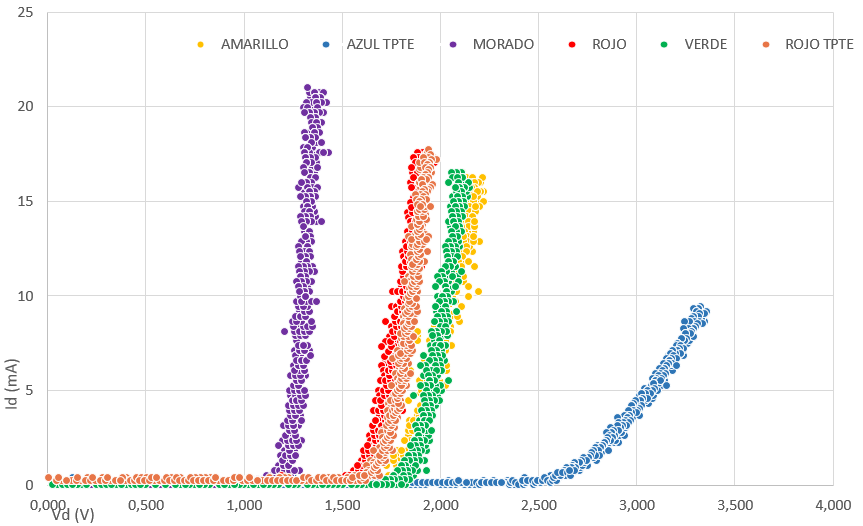
\includegraphics[scale=0.7]{capturas/diodos.png} 
	\caption{Representación de los diodos}
	\label{fig:diodos}
\end{figure}

\subsection{Diodo sin polarización, funcionando como célula fotovoltaica}

\subsubsection{Con un LED (preferentemente verde), montar el circuito de la figura, que no tiene polarización aplicada.
	Mida con el voltímetro la tensión $ V_{0} $, y verá que es mayor cuanto
	mayor sea la intensidad luminosa incidente en el LED. Parte de
	la potencia generada en el LED se pierde en el propio LED. A la
	máxima iluminación posible, calcule la potencia consumida en la
	resistencia}
\vspace{5pt}

$ R_{REAL} = 1,015 M\Omega $
\\

$ V_{0} = 0,827 V $
\\

$ P = I\cdot V_{0} = \dfrac{V_{0}^{2}}{R} = \dfrac{(0,827V)^{2}}{1015k \Omega} $ \hspace{4pt} \fboxrule=1pt \fboxsep=6pt\fbox{$ P = 0,6738 \cdot 10^{-6} W $}

\subsubsection{¿Cuántos LED serían necesarios para hacer funcionar una
	bombilla de 40W?}

$ Num_{LEDs} = 40 W \cdot \dfrac{LED}{0,6738 \cdot 10^{-6} W/LED} $ \hspace{4pt} \fboxrule=1pt \fboxsep=6pt\fbox{$ Num_{LEDs} \cong 59 \cdot 10^{6} $}

\newpage

\section{TRANSISTOR BIPOLAR DE UNIÓN}

\subsection{Curva característica de salida ($ I_{C} $ frente a $ V_{CE} $)}

\subsubsection{Con el polímetro, mida $ \beta (\beta_{F}) $ del transistor que va a usarse
	en la práctica.}

\begin{center}
	\fboxrule=1pt \fboxsep=6pt
\fbox{$ \beta (\beta_{F}) = 381 $}
\end{center}


\subsubsection{Monte el circuito de la figura. $ V_{CC} $ es una onda
triangular de 0 a 5V, y $ V_{i} $ es una tensión continua tomada de
la fuente variable de continua.}

\begin{figure}[H] %con el [H] le obligamos a situar aquí la figura
	\centering
	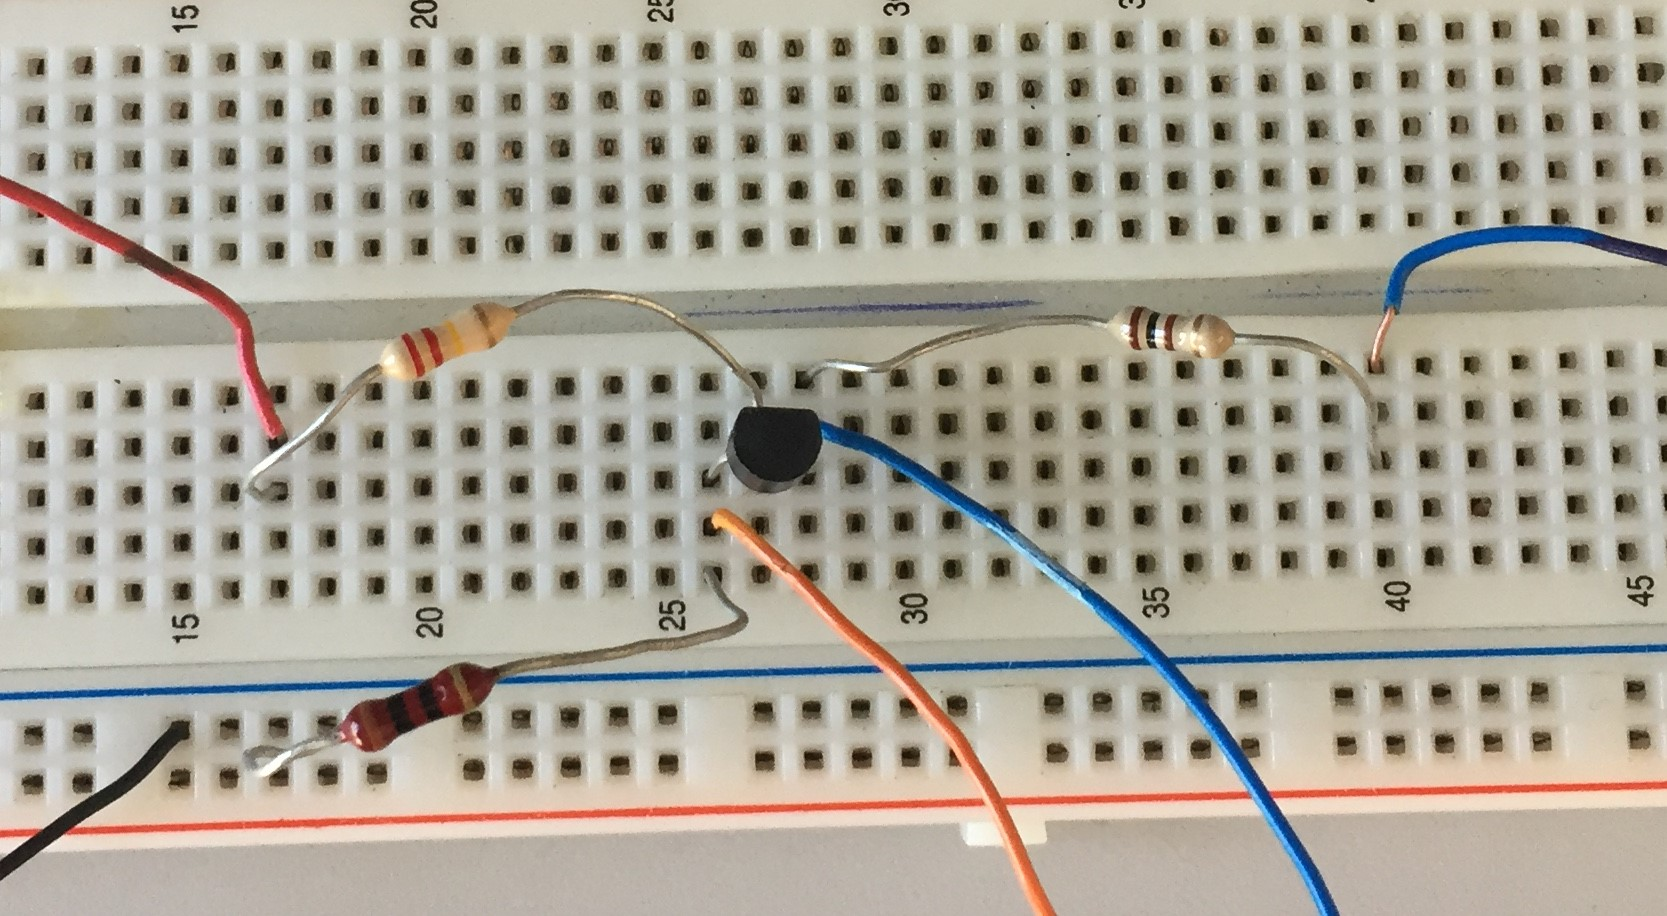
\includegraphics[scale=0.12]{capturas/4a-2.jpeg} 
	\caption{Circuito Práctica 4 - A}
	\label{fig:4a-2}
\end{figure}

\subsubsection{Conecte los canales 1 y 2 del
	osciloscopio tal como se indica en la figura.}

\begin{figure}[H] %con el [H] le obligamos a situar aquí la figura
	\centering
	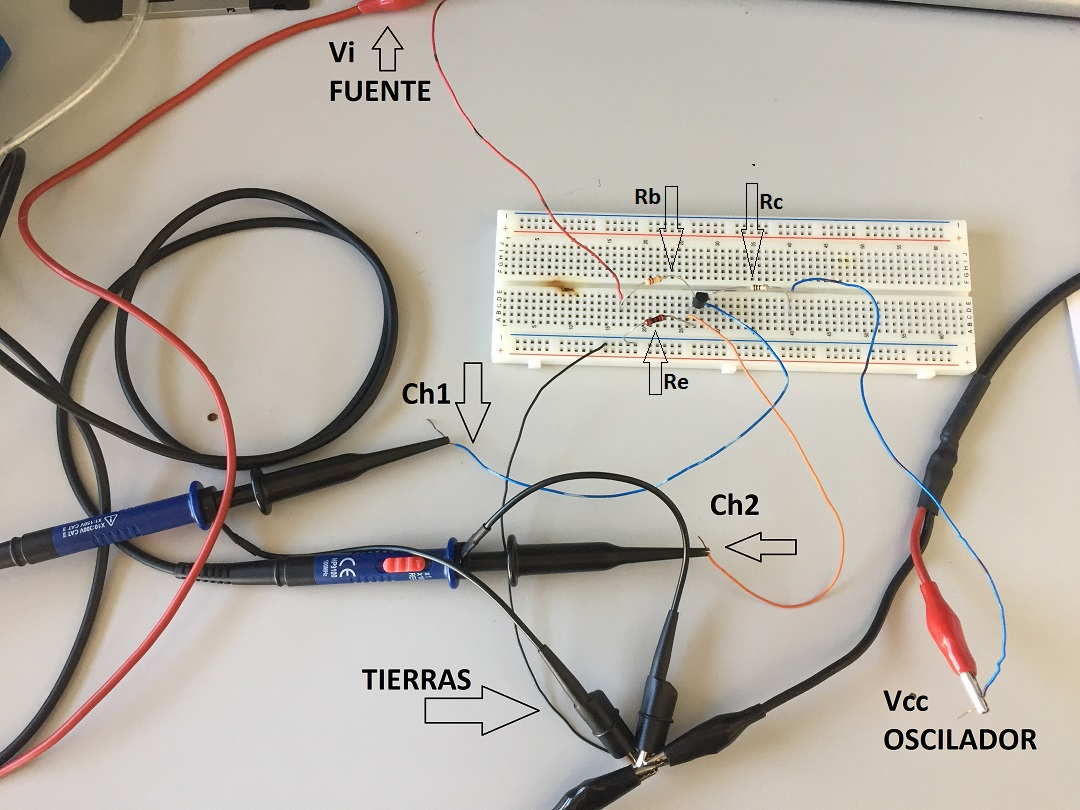
\includegraphics[scale=0.4]{capturas/4a-1.jpeg} 
	\caption{Conexiones del circuito Práctica 4 - A}
	\label{fig:4a-1}
\end{figure}

\subsubsection{Debe entregarse una gráfica con 3 curvas (como la figura, pero ésta tiene más). Las 3 curvas
	corresponderán a tres tensiones Vi de valores comprendidos entre 0,8 y 6V.}

\begin{figure}[H] %con el [H] le obligamos a situar aquí la figura
	\centering
	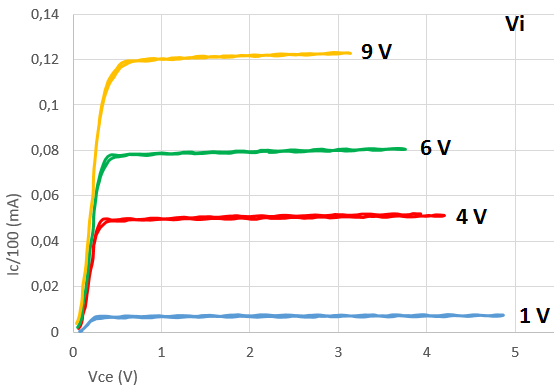
\includegraphics[scale=0.8]{capturas/practica4-graf.PNG} 
	\caption{Gráfica de las curvas Práctica 4 - A}
	\label{fig:practica4-graf}
\end{figure}


\subsubsection{Debe completarse la tabla
	asociada: $ V_{i} $ valor tomado, $ V_{BE} $ medido con el polímetro, $ V_{E} (=V_{CH2}) $ medido en ZAD con los cursores
	del osciloscopio, $ I_{E-osc} $ valor calculado como $ I_{E-osc}=V_{E}/R_{E} $, $ \beta_{osc} $ (calculado despejando $ \beta $ de la ecuación
	1, y usando la $ I_{E-osc} $)}

$ I_{E} = \dfrac{V_{i}-V_{BE}}{R_{B}+(\beta+1)\cdot R_{E} } $
\\

$ I_{E}\cdot(R_{B}+\beta R_{E} +  R_{E} ) = \beta \cdot(V_{i}-V_{BE}) +  (V_{i}-V_{BE})$
\\

$ \beta = \dfrac{I_{E}\cdot R_{B} + I_{E}\cdot R_{E} - (V_{i}-V_{BE})}{(V_{i}-V_{BE}) - I_{E}\cdot R_{E}} $

% Table generated by Excel2LaTeX from sheet ,Hoja1,
\begin{table}[htbp]
	\centering
	\begin{tabular}{rrrrr}
		\multicolumn{1}{l}{\textbf{$ V_{i} $ }} & \multicolumn{1}{l}{\textbf{$ V_{BE} $ }} & \multicolumn{1}{l}{\textbf{$ V_{E} $ }} & \multicolumn{1}{l}{\textbf{$ I_{E-osc} $ }} & \multicolumn{1}{l}{\textbf{$ \beta_{osc} $}} \\
		\midrule
		1     & 0,58  & 0,00688 & 0,688 & 365,3826 \\
		4     & 0,67  & 0,05125 & 5,125 & 342,8811 \\
		6     & 0,685 & 0,07937 & 7,937 & 332,511 \\
		9     & 0,69  & 0,1219 & 12,19 & 326,5241 \\
	\end{tabular}%	
	\caption{Tabla asociada a la curva característica de salida}
	\label{tab:tabla4a}%
\end{table}%

Con los datos de la gráfica, se ha obtenido una media de 341, cuando polímetro medía 381. Por tanto, \textbf{el error es de un 11\%}.


\newpage


\subsection{Montaje amplificador básico. Cálculo de la ganancia}

\subsubsection{Montaje del circuito}

\begin{figure}[H] %con el [H] le obligamos a situar aquí la figura
	\centering
	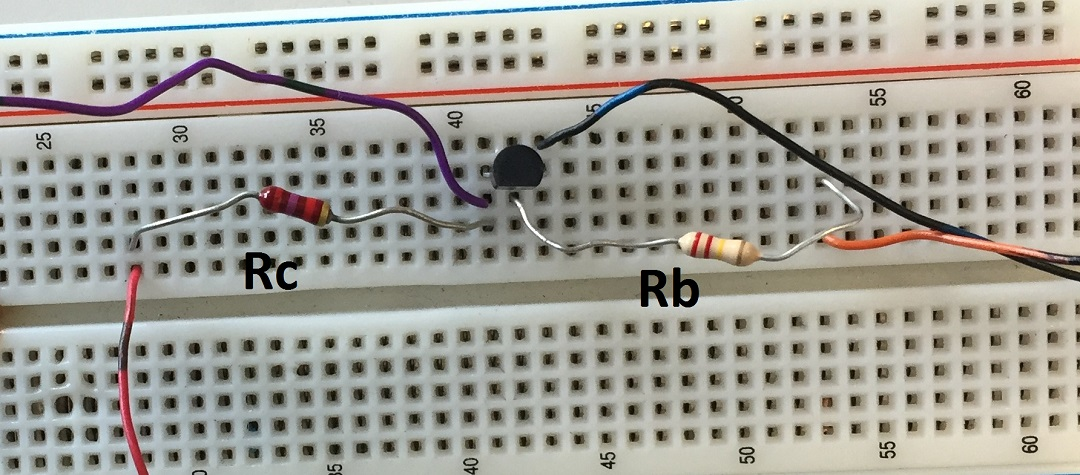
\includegraphics[scale=0.4]{capturas/ejercicio4/figura1.jpg} 
	\caption{Montaje del circuito}
	\label{fig:practica4-b-1}
\end{figure}

\subsubsection{Conexiones del circuito}

\begin{figure}[H] %con el [H] le obligamos a situar aquí la figura
	\centering
	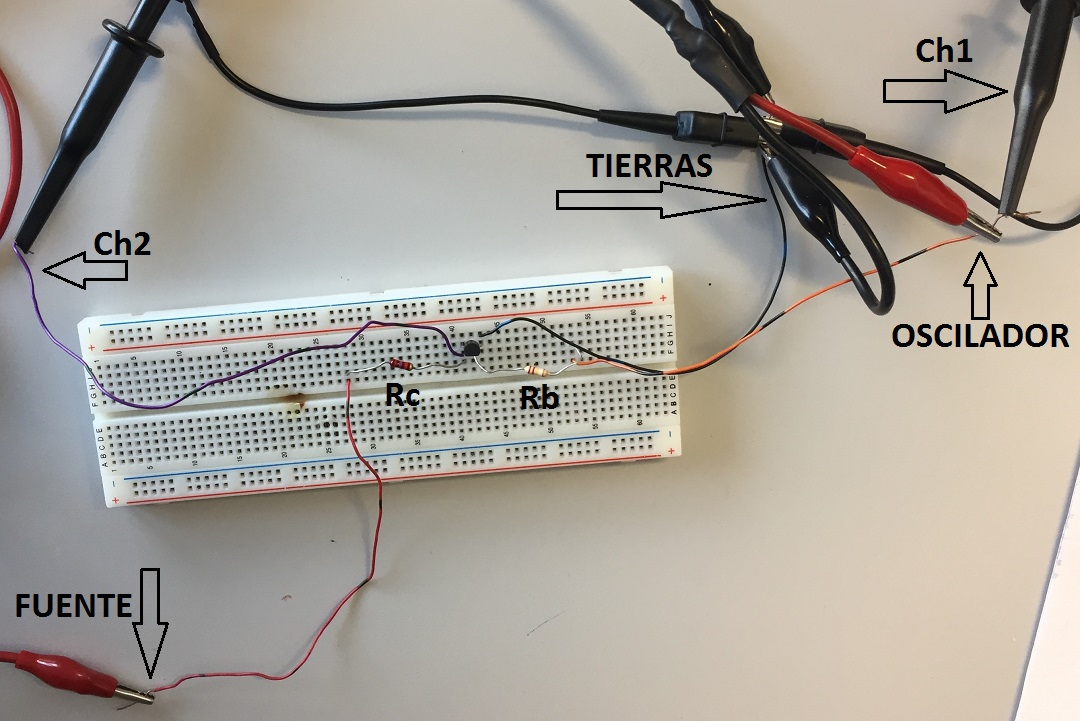
\includegraphics[scale=0.4]{capturas/ejercicio4/figura2.jpg} 
	\caption{Montaje del circuito}
	\label{fig:practica4-b-2}
\end{figure}


\subsubsection{Deberán tomarse cuatro medidas distintas de la ganancia. La primera será con un valor $ V_{DC}=0,8V $, la
	última con el valor $ V_{DC} $ que haga visible en $ v_{o} $ que el transistor entra en saturación, otra en el $ V_{DC} $ que
	dé la máxima ganancia, y una cuarta donde se quiera.
	Deberán entregarse las imágenes (TIF) de esas cuatro medidas, y rellenar la siguiente tabla}
\vspace{-20pt}
% Table generated by Excel2LaTeX from sheet ,Hoja1,
\begin{table}[H]
	\centering
	\caption{Medidas con $ V_{DC} = 0,8 V $}
	\begin{tabular}{rrrrl}
		\multicolumn{1}{l}{\textbf{$ V_{DC} $}} & \multicolumn{1}{l}{\textbf{$ v_{i} $}} & \multicolumn{1}{l}{\textbf{$ v_{o} $}} & \multicolumn{1}{l}{\textbf{$ v_{o}/v_{i} $}} & \textbf{Comentario} \\
		\midrule
		\textbf{0,8}   & 199   & 708   & 3,557789 & Crecimiento inicial  \\
	\end{tabular}%
	\label{tab:p4b1}%
\end{table}%
\vspace{-20pt}
\begin{figure}[H] %con el [H] le obligamos a situar aquí la figura
	\centering
	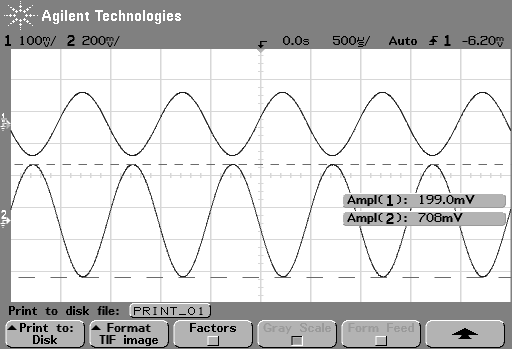
\includegraphics[scale=0.7]{capturas/ejercicio4/B/PRINT_01.png} 
	\caption{Imagen para las medidas con $ V_{DC} = 0,8 V $}
	\label{fig:practica4-b-3}
\end{figure}
\vspace{-20pt}
------------------------------------------------------------------------------------------------------------------
\vspace{-15pt}
\begin{table}[H]
	\centering
	\caption{Medidas con $ V_{DC} = 1 V $}
	\begin{tabular}{rrrrl}
		\multicolumn{1}{l}{\textbf{$ V_{DC} $}} & \multicolumn{1}{l}{\textbf{$ v_{i} $}} & \multicolumn{1}{l}{\textbf{$ v_{o} $}} & \multicolumn{1}{l}{\textbf{$ v_{o}/v_{i} $}} & \textbf{Comentario} \\
		\midrule
		\textbf{1}     & 199   & 752   & 3,778894 & Cerca de ganancia máxima 
		 \\
	\end{tabular}%
	\label{tab:p4b2}%
\end{table}%
\vspace{-20pt}
\begin{figure}[H] %con el [H] le obligamos a situar aquí la figura
	\centering
	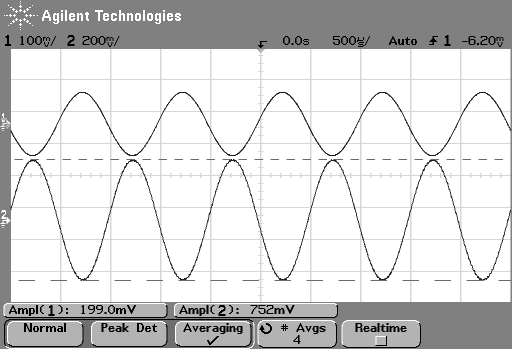
\includegraphics[scale=0.7]{capturas/ejercicio4/B/PRINT_05.png} 
	\caption{Imagen para las medidas con $ V_{DC} = 1 V $}
	\label{fig:practica4-b-4}
\end{figure}

\begin{table}[H]
	\centering
	\caption{Medidas con $ V_{DC} = 1,39 V $}
	\begin{tabular}{rrrrl}
		\multicolumn{1}{l}{\textbf{$ V_{DC} $}} & \multicolumn{1}{l}{\textbf{$ v_{i} $}} & \multicolumn{1}{l}{\textbf{$ v_{o} $}} & \multicolumn{1}{l}{\textbf{$ v_{o}/v_{i} $}} & \textbf{Comentario} \\
		\midrule
		\textbf{1,39}  & 199,8 & 761   & 3,808809 & Ganancia máxima 
		\\
	\end{tabular}%
	\label{tab:p4b3}%
\end{table}%
\vspace{-20pt}
\begin{figure}[H] %con el [H] le obligamos a situar aquí la figura
	\centering
	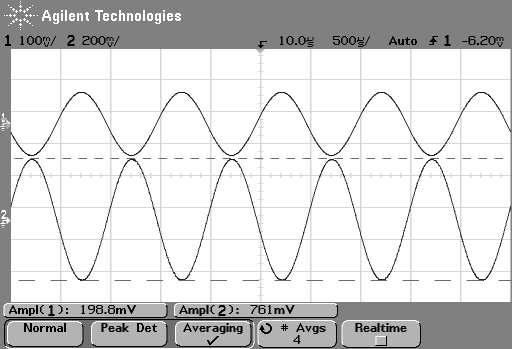
\includegraphics[scale=0.75]{capturas/ejercicio4/B/PRINT_06.png} 
	\caption{Imagen para las medidas con $ V_{DC} = 1,39 V $}
	\label{fig:practica4-b-5}
\end{figure}
\vspace{-20pt}
------------------------------------------------------------------------------------------------------------------
\vspace{-15pt}
\begin{table}[H]
	\centering
	\caption{Medidas con $ V_{DC} = 1,8 V $}
	\begin{tabular}{rrrrl}
		\multicolumn{1}{l}{\textbf{$ V_{DC} $}} & \multicolumn{1}{l}{\textbf{$ v_{i} $}} & \multicolumn{1}{l}{\textbf{$ v_{o} $}} & \multicolumn{1}{l}{\textbf{$ v_{o}/v_{i} $}} & \textbf{Comentario} \\
		\midrule
		\textbf{1,8}   & 199,4 & 700   & 3,510532 & Entra en saturación \\
	\end{tabular}%
	\label{tab:p4b4}%
\end{table}%
\vspace{-20pt}
\begin{figure}[H] %con el [H] le obligamos a situar aquí la figura
	\centering
	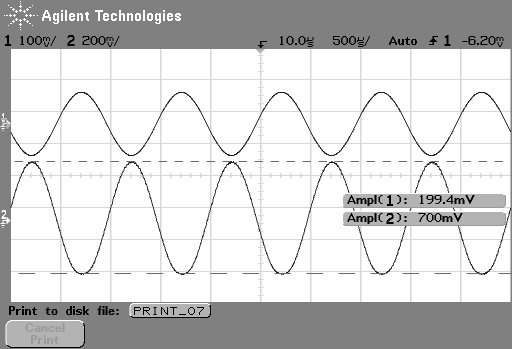
\includegraphics[scale=0.75]{capturas/ejercicio4/B/PRINT_07.png} 
	\caption{Imagen para las medidas con $ V_{DC} = 1,8 V $}
	\label{fig:practica4-b-6}
\end{figure}

\newpage
Tabla con todas las medidas:

\begin{table}[H]
	\centering
	\begin{tabular}{rrrrl}
		\multicolumn{1}{l}{\textbf{$ V_{DC} $}} & \multicolumn{1}{l}{\textbf{$ v_{i} $}} & \multicolumn{1}{l}{\textbf{$ v_{o} $}} & \multicolumn{1}{l}{\textbf{$ v_{o}/v_{i} $}} & \textbf{Comentario} \\
		\midrule
		\textbf{0,8}   & 199   & 708   & 3,557789 & Crecimiento inicial \\
		\textbf{1}     & 199   & 752   & 3,778894 & Cerca de ganancia máxima \\
		\textbf{1,39}  & 199,8 & 761   & 3,808809 & Ganancia máxima \\
		\textbf{1,8}   & 199,4 & 700   & 3,510532 & Entra en saturación \\
	\end{tabular}%
	\caption{Medidas Práctica 4 - B}
	\label{tab:p4b}%
\end{table}%

\section{FAMILIAS LÓGICAS: CMOS}

\subsection{Puerta NOT CMOS}

\subsubsection{Construir la puerta NOT. Comprobar que los niveles de tensión de la tabla de verdad son correctos}

\begin{figure}[H] %con el [H] le obligamos a situar aquí la figura
	\centering
	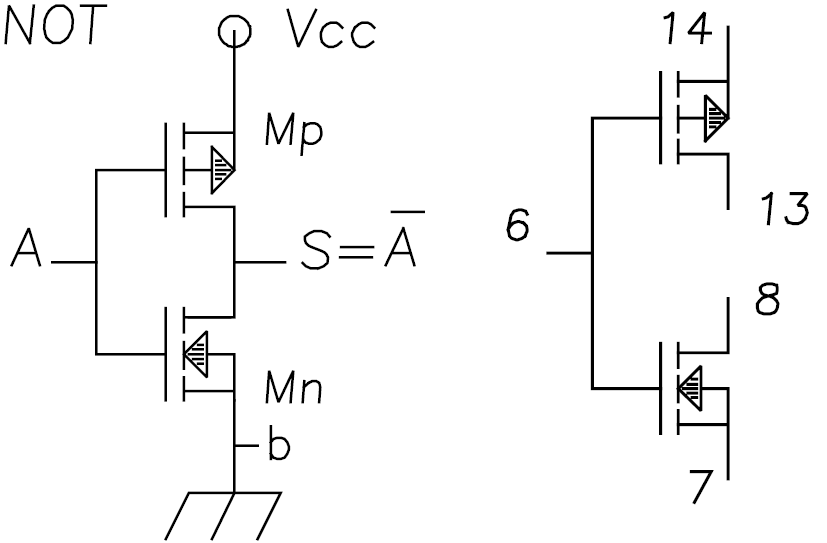
\includegraphics[scale=0.35]{capturas/ejercicio5/A/teo.png} 
	\caption{Puerta NOT a realizar}
	\label{fig:practica5-a-1}
\end{figure}
\vspace{-15pt}
\begin{figure}[H] %con el [H] le obligamos a situar aquí la figura
	\centering
	\includegraphics[scale=0.5]{capturas/ejercicio5/A/figura1.png} 
	\caption{Puerta NOT a realizar}
	\label{fig:practica5-a-2}
\end{figure}

\begin{figure}[H] %con el [H] le obligamos a situar aquí la figura
	\centering
	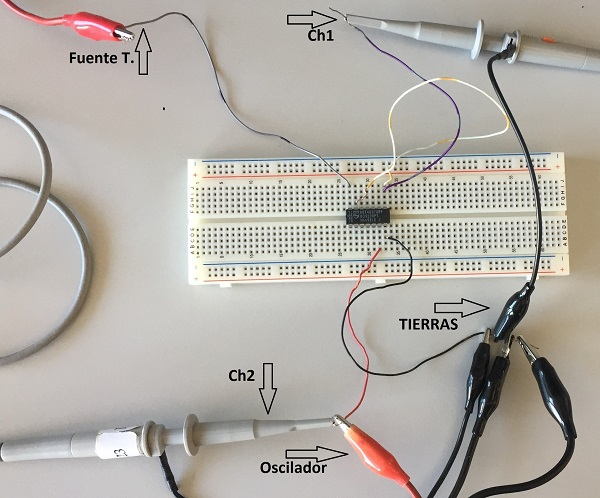
\includegraphics[scale=0.7]{capturas/ejercicio5/A/figura2.jpg} 
	\caption{Conexiones de la puerta NOT CMOS}
	\label{fig:practica5-a-3}
\end{figure}

Los niveles de tensión de la tabla de verdad son correctos porque para valores de entrada grandes, aparecen valores bajos y viceversa como puede verse en la Figura \ref{fig:practica5-a-4}.

\textbf{Alimentación = 8V}
\begin{figure}[H] %con el [H] le obligamos a situar aquí la figura
	\centering
	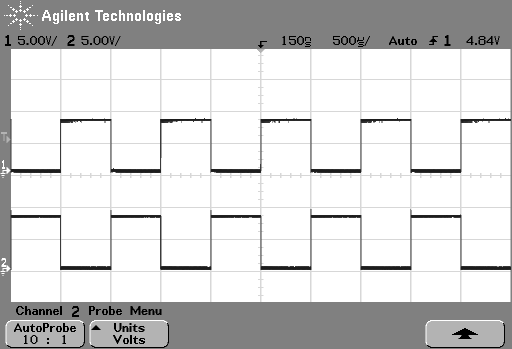
\includegraphics[scale=0.7]{capturas/ejercicio5/A/PRINT00.png} 
	\caption{Resultados del apartado uno}
	\label{fig:practica5-a-4}
\end{figure}


\subsubsection{Apuntar la máxima frecuencia de trabajo admisible. Medir los retardos de bajo-alto y de alto-bajo}

No existe una máxima frecuencia de trabajo, solamente hay que tenerlo en cuenta en función de la utilidad final que se le quiera dar. Por ejemplo, en este caso (Figura \ref{fig:practica5-a-5}) se ha llegado a una frecuencia de 10MHz, con los inconvenientes que conlleva una alta frecuencia pero lo ha logrado.


\begin{figure}[H] %con el [H] le obligamos a situar aquí la figura
	\centering
	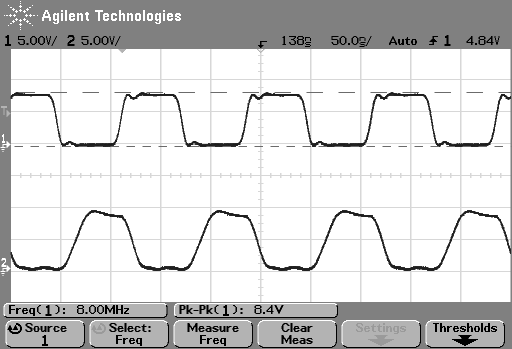
\includegraphics[scale=0.7]{capturas/ejercicio5/A/PRINT01.png} 
	\caption{Resultados del apartado dos}
	\label{fig:practica5-a-5}
\end{figure}

Retardo bajo-alto: 8,40ns

\begin{figure}[H] %con el [H] le obligamos a situar aquí la figura
	\centering
	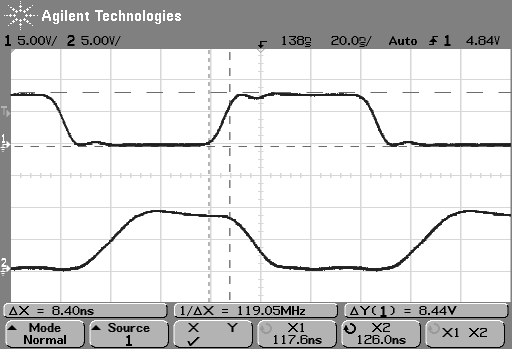
\includegraphics[scale=0.7]{capturas/ejercicio5/A/PRINT02.png} 
	\caption{Retardo bajo-alto}
	\label{fig:practica5-a-6}
\end{figure}

\newpage

Retardo alto-bajo: 12ns

\begin{figure}[H] %con el [H] le obligamos a situar aquí la figura
	\centering
	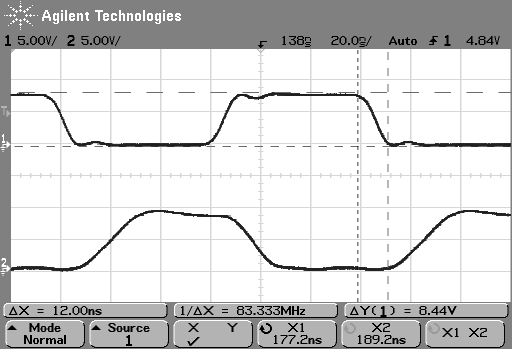
\includegraphics[scale=0.8]{capturas/ejercicio5/A/PRINT03.png} 
	\caption{Retardo alto-bajo}
	\label{fig:practica5-a-7}
\end{figure}

\subsubsection{Con una señal triangular ($ \sim $1 kHz), medir la tensión umbral ($ V_{T} $)}

$ V_{T} = 3.938 V $

\begin{figure}[H] %con el [H] le obligamos a situar aquí la figura
	\centering
	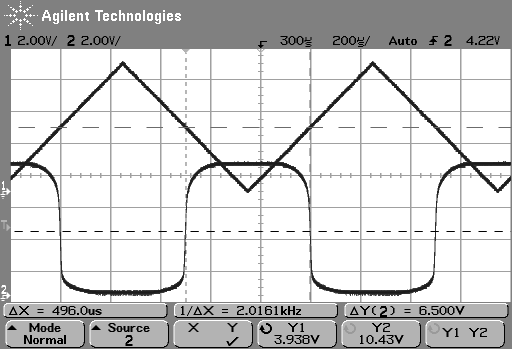
\includegraphics[scale=0.8]{capturas/ejercicio5/A/PRINT04.png} 
	\caption{Tensión umbral}
	\label{fig:practica5-a-8}
\end{figure}

\newpage

\subsubsection{Con la anterior señal triangular, poner el modo XY del osciloscopio (Ch1 en
	A, Ch2 en S). Dibujar la función de transferencia.}

\begin{figure}[H] %con el [H] le obligamos a situar aquí la figura
	\centering
	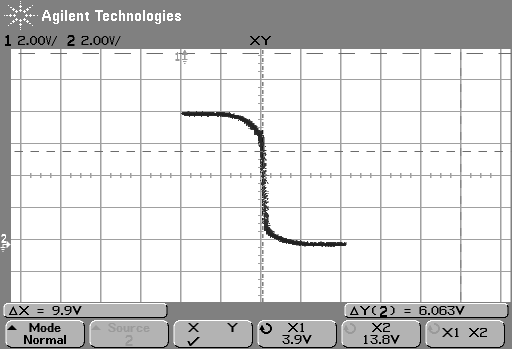
\includegraphics[scale=0.8]{capturas/ejercicio5/A/PRINT05.png} 
	\caption{Función de transferencia}
	\label{fig:practica5-a-9}
\end{figure}

\subsubsection{Añadir una resistencia de bajo
	valor (~100 W) entre b y tierra. Con el osciloscopio en modo XY (Ch1 en A, Ch2
	en b) dibujar la gráfica de consumo de la puerta CMOS.}

\begin{figure}[H] %con el [H] le obligamos a situar aquí la figura
	\centering
	\includegraphics[scale=0.6]{capturas/ejercicio5/A/figura3.png} 
	\caption{Añadido de resistencia sobre NOT CMOS}
	\label{fig:practica5-a-10}
\end{figure}

\begin{figure}[H] %con el [H] le obligamos a situar aquí la figura
	\centering
	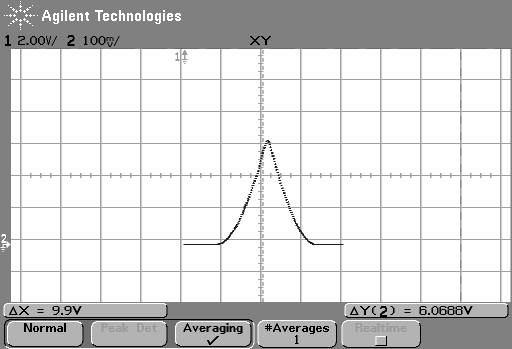
\includegraphics[scale=0.8]{capturas/ejercicio5/A/PRINT06.png} 
	\caption{Gráfica de consumo de la puerta CMOS}
	\label{fig:practica5-a-11}
\end{figure}

\subsection{Memoria CMOS}

\subsubsection{Montar la célula de memoria CMOS de la figura, con entrada A y salidas S’ y S}

Se ha establecido el patillaje del circuito atendiendo a la numeración que se encuentra de color rojo en la Figura \ref{fig:practica5-a-12}.

\begin{figure}[H] %con el [H] le obligamos a situar aquí la figura
	\centering
		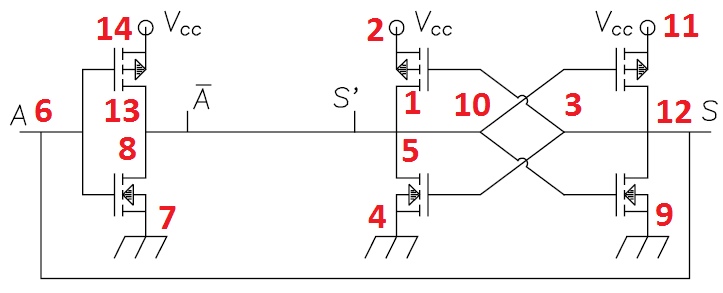
\includegraphics[scale=0.7]{capturas/ejercicio5/B/figura4.png} 
	\caption{Numeración del patillaje en la Memoria CMOS}
	\label{fig:practica5-a-12}
\end{figure}

\begin{figure}[H] %con el [H] le obligamos a situar aquí la figura
	\centering
	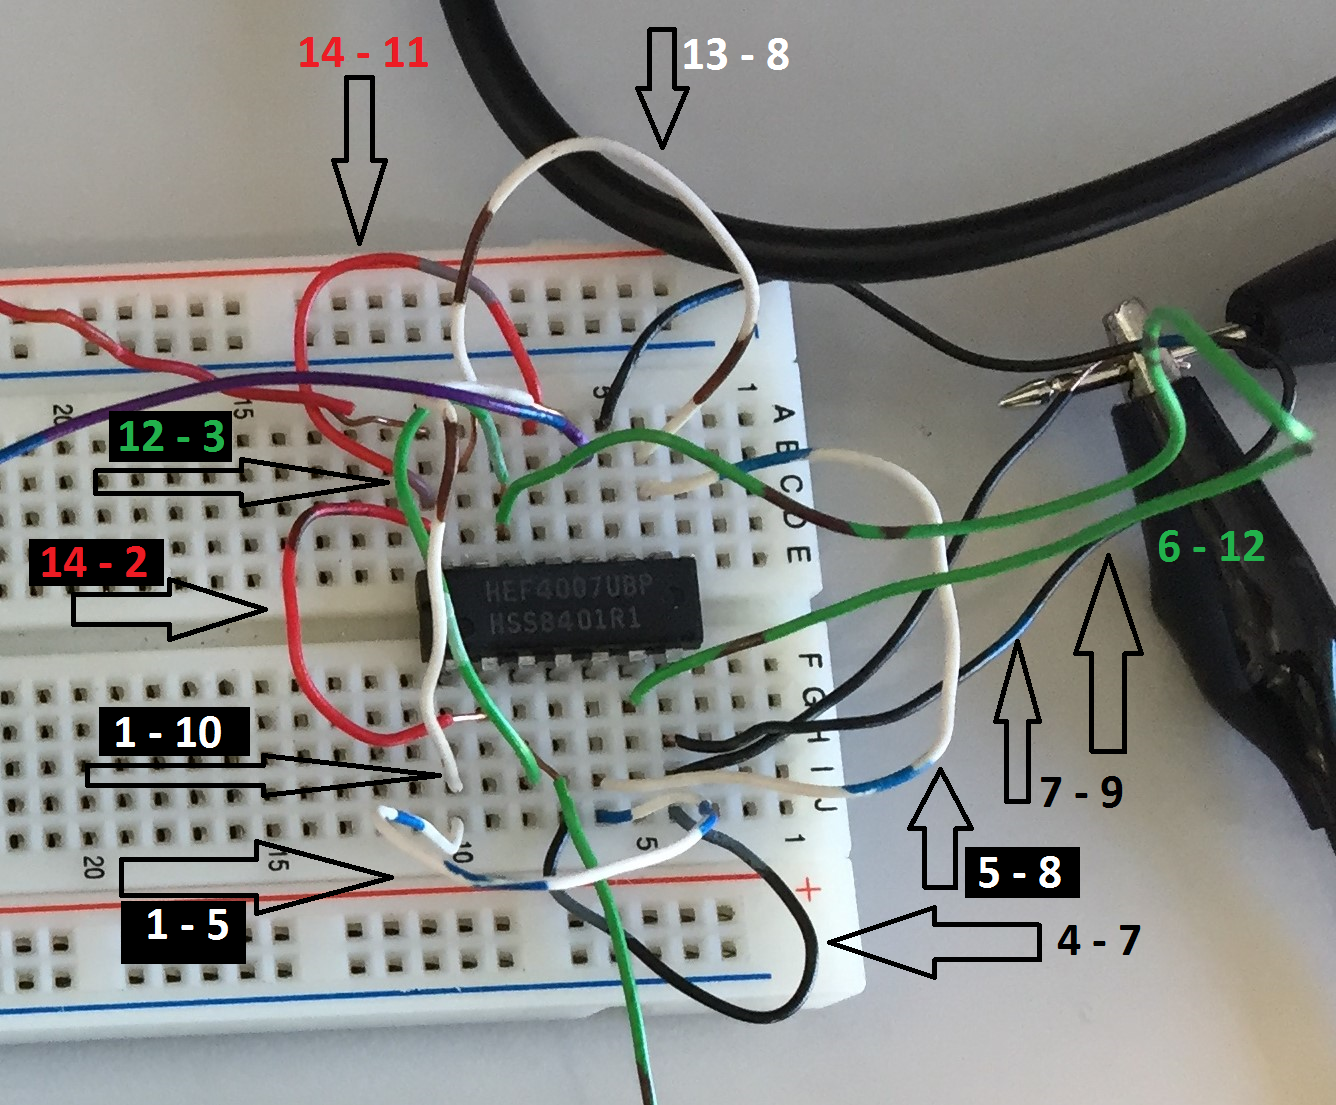
\includegraphics[scale=0.25]{capturas/ejercicio5/B/figura2.png} 
	\caption{Numeración del patillaje en el circuito de la Memoria CMOS}
	\label{fig:practica5-a-13}
\end{figure}

\begin{figure}[H] %con el [H] le obligamos a situar aquí la figura
	\centering
	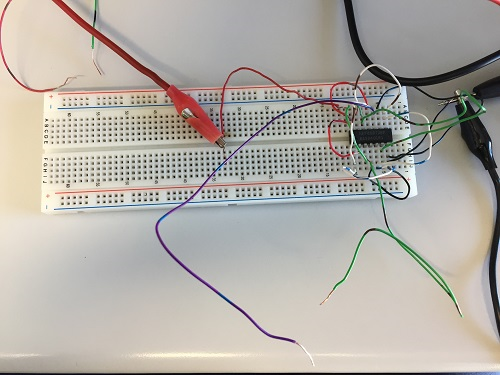
\includegraphics[scale=0.8]{capturas/ejercicio5/B/figura1.png} 
	\caption{Circuito de Memoria CMOS}
	\label{fig:practica5-a-14}
\end{figure}

\newpage

\subsubsection{Con A=0, comprobar que las salidas S’ y S son correctas. Desconectar A y comprobar que S’ y S se
	mantienen en sus valores correctos.}
 
% Table generated by Excel2LaTeX from sheet ,Hoja1,
\begin{table}[H]
	\centering
	\begin{tabular}{l|rr|rrr}
		& \textbf{S, = \={A} } & \textbf{¿Medir?} & \textbf{S = A} & \textbf{¿Medir?} & \textbf{¿Retiene valor previo?}\\
		\midrule
		\textbf{A = 0} & 1     & SI    & 0     & NO \\
		\textbf{Desconecto A} & 1     & SI    & 0     & SI & SI\\
	\end{tabular}%
	\caption{Salidas cuando A=0}
	\label{tab:ejercicio5b-1}%
\end{table}%



\subsubsection{Con A=1, comprobar que las salidas S’ y S son correctas. Desconectar A y comprobar que S’ y S se
	mantienen en sus valores correctos}

% Table generated by Excel2LaTeX from sheet ,Hoja1,
\begin{table}[H]
	\centering
	\begin{tabular}{l|rr|rrr}
		& \textbf{S, = \={A} } & \textbf{¿Medir?} & \textbf{S = A} & \textbf{¿Medir?} & \textbf{¿Retiene valor previo?}\\
		\midrule
		\textbf{A = 1} & 0     & SI    & 1     & NO \\
		\textbf{Desconecto A} & 0     & SI    & 1     & SI & SI \\
	\end{tabular}%
	\caption{Salidas cuando A=1}
	\label{tab:ejercicio5b-2}%
\end{table}%

\section{CONVERSOR ANALOGICO-DIGITAL}

\subsection{Medir la tensión de alimentación $ V_{DD} $ de forma muy precisa
	y calcular el valor del LSB (LSB= REF / 1024).}
$ V_{DD} = 5,010 V$\\

$ LSB = REF / 1024 = 5,011 V / 1024 = 4,893554688mV$
\subsection{Para cada tensión analógica:}
	\subsubsection{Para 1,8V de Variable}
		\begin{itemize}
			\item Se mide, de forma muy precisa, la tensión de entrada analógica $ V_{a} $
			
			$ V_{a} = 1,9076 V$
			\item Se captura en un disquete la imagen (tif o bmp) del osciloscopio (datos y reloj).
				\begin{figure}[H] %con el [H] le obligamos a situar aquí la figura
					\centering
					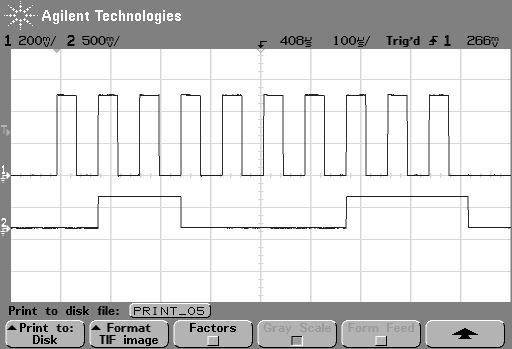
\includegraphics[scale=0.6]{capturas/ejercicio6/PRINT05.png} 
					\caption{Tensión de entrada para 1,8V de Variable}
					\label{fig:practica6-1}
				\end{figure}
			\item Se extrae de la imagen, la palabra numérica (en binario) y se convierte a decimal.
			
				En la Figura  \ref{fig:practica6-1}, se ve que hay 10 pulsos de reloj. En la línea de datos (la de abajo) aparecen los 10 bits de la conversión
				analógico-digital. Aparece primero el bit más significativo (MSB), y se termina por el menos significativo (LSB).\\
				
				La palabra numérica
				correspondiente a la tensión analógica de entrada $ V_{a} = 1,9076 V$ resulta ser \textbf{1 1000 0111}, es decir \textbf{391 en decimal}.
			
			\item Se comprueba que la palabra digital se corresponde con el valor teórico dado por la siguiente
			ecuación (E= función parte entera, Min= función mínimo):
			
				\begin{center}
					$ Num(V_{a}) = Min [E(\dfrac{V_{a} + \frac{LSB}{2}}{LSB})]$
				\end{center}
			
				$ Num(V_{a}) = Min [E(\dfrac{1907,6mV + \frac{4,893554688mV}{2}}{4,893554688mV})] $ \hspace{3pt} {\fboxrule=1pt \fboxsep=6pt
					\fbox{$ Num = 390 $}}			
		\end{itemize}
	
	\subsubsection{Para 1,1V de Variable}
		\begin{itemize}
			\item Se mide, de forma muy precisa, la tensión de entrada analógica $ V_{a} $
			
			$ V_{a} = 1,1913 V$
			\item Se captura en un disquete la imagen (tif o bmp) del osciloscopio (datos y reloj).
			\begin{figure}[H] %con el [H] le obligamos a situar aquí la figura
				\centering
				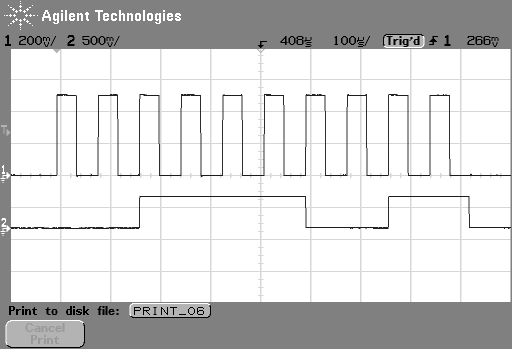
\includegraphics[scale=0.7]{capturas/ejercicio6/PRINT06.png} 
				\caption{Tensión de entrada para 1,1V de Variable}
				\label{fig:practica6-2}
			\end{figure}
			\item Se extrae de la imagen, la palabra numérica (en binario) y se convierte a decimal.
			
			En la Figura  \ref{fig:practica6-2}, se ve que hay 10 pulsos de reloj. En la línea de datos (la de abajo) aparecen los 10 bits de la conversión
			analógico-digital. Aparece primero el bit más significativo (MSB), y se termina por el menos significativo (LSB).\\
			
			La palabra numérica
			correspondiente a la tensión analógica de entrada $ V_{a} = 1,1913 V$ resulta ser \textbf{1111 0011}, es decir \textbf{243 en decimal}.
			
			\item Se comprueba que la palabra digital se corresponde con el valor teórico dado por la siguiente
			ecuación (E= función parte entera, Min= función mínimo):
			
			\begin{center}
				$ Num(V_{a}) = Min [E(\dfrac{V_{a} + \frac{LSB}{2}}{LSB})]$
			\end{center}
			
			$ Num(V_{a}) = Min [E(\dfrac{1191,3mV + \frac{4,893554688mV}{2}}{4,893554688mV})] $ \hspace{3pt} {\fboxrule=1pt \fboxsep=6pt
				\fbox{$ Num = 243 $}}			
		\end{itemize}
	
	\subsubsection{Para 0,4V de Variable}
	\begin{itemize}
		\item Se mide, de forma muy precisa, la tensión de entrada analógica $ V_{a} $
		
		$ V_{a} = 0,4635 V$
		\item Se captura en un disquete la imagen (tif o bmp) del osciloscopio (datos y reloj).
		\begin{figure}[H] %con el [H] le obligamos a situar aquí la figura
			\centering
			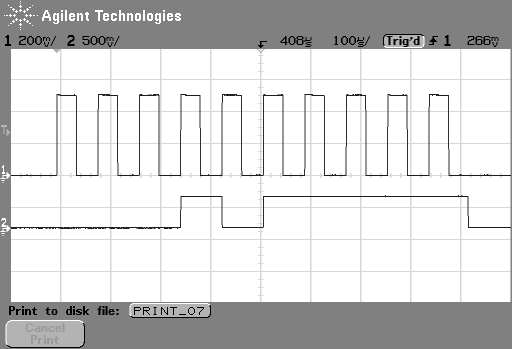
\includegraphics[scale=0.7]{capturas/ejercicio6/PRINT07.png} 
			\caption{Tensión de entrada para 0,4V de Variable}
			\label{fig:practica6-3}
		\end{figure}
		\item Se extrae de la imagen, la palabra numérica (en binario) y se convierte a decimal.
		
		En la Figura  \ref{fig:practica6-3}, se ve que hay 10 pulsos de reloj. En la línea de datos (la de abajo) aparecen los 10 bits de la conversión
		analógico-digital. Aparece primero el bit más significativo (MSB), y se termina por el menos significativo (LSB).\\
		
		La palabra numérica
		correspondiente a la tensión analógica de entrada $ V_{a} = 0,4635 V$ resulta ser \textbf{101 1111}, es decir \textbf{95 en decimal}.
		
		\item Se comprueba que la palabra digital se corresponde con el valor teórico dado por la siguiente
		ecuación (E= función parte entera, Min= función mínimo):
		
		\begin{center}
			$ Num(V_{a}) = Min [E(\dfrac{V_{a} + \frac{LSB}{2}}{LSB})]$
		\end{center}
		
		$ Num(V_{a}) = Min [E(\dfrac{463,5mV + \frac{4,893554688mV}{2}}{4,893554688mV})] $ \hspace{3pt} {\fboxrule=1pt \fboxsep=6pt
			\fbox{$ Num = 95 $}}			
	\end{itemize}

\end{document}
